% Paper v4: optimizer-first narrative revision.
% Build: PATH="/opt/texlive/2026/bin/x86_64-linux:$PATH" latexmk -pdf -interaction=nonstopmode -halt-on-error main.tex
\ifdefined\pdftexversion\pdfoutput=1\fi
\documentclass[11pt]{article}

\usepackage[utf8]{inputenc}
\usepackage[T1]{fontenc}
\usepackage[margin=1in, top=1.1in, bottom=0.8in]{geometry}
\setlength{\skip\footins}{30pt}
\usepackage{amsmath, amssymb, amsfonts, amsthm, mathtools}
\usepackage{graphicx}
\usepackage{booktabs}
\usepackage{array}
\usepackage{tabularx}
\usepackage{longtable,placeins}
\usepackage{microtype}
\usepackage[table]{xcolor}
\usepackage[authoryear, sort&compress, round]{natbib}
\PassOptionsToPackage{hyphens}{url}
\usepackage{xurl}
\usepackage[colorlinks, pagebackref, linktoc=page]{hyperref}
\usepackage[nameinlink, capitalize]{cleveref}
\usepackage{paperstyle}

\crefname{equation}{}{}
\crefformat{section}{\S#2#1#3}
\crefformat{appendix}{\S#2#1#3}
\crefname{figure}{Figure}{Figures}
\Crefname{figure}{Figure}{Figures}
\captionsetup{width=\textwidth}
\hypersetup{hypertexnames=false}
\setlength{\headsep}{15pt}

\pagestyle{paper}
\papershorttitle{Structure-aware two-sided preconditioning for Muon}
\graphicspath{{figs/}}
\urlstyle{tt}
\interfootnotelinepenalty=10000

\renewcommand{\topfraction}{0.85}
\renewcommand{\bottomfraction}{0.80}
\renewcommand{\textfraction}{0.08}
\renewcommand{\floatpagefraction}{0.80}

% Mathematical notation macros
\newcommand{\Tr}{{\mathsf{T}}}
\newcommand{\Nten}{\mathcal{N}_{10}}
\newcommand{\unitrms}{\operatorname{unitRMS}}
\newcommand{\tr}{\operatorname{tr}}
\newcommand{\Diag}{\operatorname{Diag}}
\newcommand{\diag}{\operatorname{diag}}
\newcommand{\E}{\mathbb{E}}
\newcommand{\R}{\mathbb{R}}
\newcommand{\dm}{d_{\mathrm{model}}}
\newcommand{\dff}{d_{\mathrm{ff}}}
\newcommand{\Lsel}{\mathcal{L}_{\mathrm{sel}}}
\newcommand{\Lc}{\mathcal{L}_{\mathrm{C4}}}
\newcommand{\Lpal}{\mathcal{L}_{\mathrm{Paloma}}}

% Consistent method names
\newcommand{\mname}[1]{#1}
\definecolor{colWT}{HTML}{1B4F9C}
\definecolor{colOD}{HTML}{0E7C7B}
\definecolor{colNull}{HTML}{C87D20}
\definecolor{colBad}{HTML}{C0392B}
\definecolor{rowtint}{HTML}{F2F6FC}

\title{Structure-Aware Two-Sided\\Preconditioning for Muon Optimizers}
\author{Optimizer Research Team}
\paperaffiliations{Preprint}

\begin{document}

\maketitle

\begin{abstract}
\mname{Muon} orthogonalizes matrix momentum with Newton--Schulz iterations, and \mname{MuonT} lowers Transformer pretraining loss by preconditioning on input activations alone. Extending \mname{MuonT} to backpropagated output cotangents is costly if done densely at every layer (\mname{Muon2-Dense}), because cubic eigendecompositions sit at the end of backpropagation; yet purely diagonal output scaling (\mname{Muon2-Diag}) misses cross-channel correlations, adding little held-out benefit and falling behind \mname{MuonT} out of distribution on wider models. We introduce \mname{Muon2-ExpDiag}, a structure-aware two-sided preconditioned Muon optimizer that pairs \mname{MuonT}'s dense input factors and right-only weight decay ($W\hat R^2$) with expansion-diagonal output factors and a one-step lag. \mname{Muon2-ExpDiag} applies dense $(-1/2,-1/8)$ inverse roots to the five hidden-width outputs ($\dm$: \texttt{q,k,v,o,down}), exact per-step diagonal scaling to the two gated SwiGLU expansion outputs ($\dff=4\dm$: \texttt{gate,up}), and asynchronous background root updates overlapped with the next training step. Across audited trajectories, expanded SwiGLU outputs account for 96.2\% of nominal dense output eigendecomposition work while carrying 78--91\% of their anisotropy on the coordinate diagonal, whereas residual-stream outputs (\texttt{o,down}) carry over 99\% of their anisotropy in cross-channel correlations and rotate eigenspaces far faster than RMSNormed inputs. Relative to tuned \mname{MuonT}, \mname{Muon2-ExpDiag} lowers final held-out loss by 0.0035 nats across three 130M seeds, 0.0040 nats at four times the token budget, and 0.0046 nats at 520M, extending \mname{MuonT}'s improvement over \mname{Muon} by 29--51\%. The longer and wider runs each use one seed. Multi-seed ablations confirm that right-only weight decay outperforms both isotropic ($W$) and two-sided ($\hat L^2 W\hat R^2$) decay across held-out, C4, and Paloma evaluations. Checkpoint probes further show that dense output factors rotate residual updates without inflating step norms and cut leading output-subspace drift by 17--21\% relative to \mname{Muon}. Relative to \mname{Muon}, median step-time overhead is 6.8\% at 130M and 8.2\% at 520M (5.3\% and 3.3\% above \mname{MuonT}), with mean overheads of 10.7\% and 17.0\% (8.9\% and 11.4\% above \mname{MuonT}), establishing a fixed-token loss improvement at a modest throughput cost.
\end{abstract}

\section{Introduction}
\label{sec:intro}

\paragraph{The output-preconditioning dilemma.}
\mname{Muon} maps matrix momentum toward a semi-orthogonal update using Newton--Schulz iterations~\citep{jordan2024muon}, and \mname{MuonT} (also called Toner) lowers Transformer pretraining loss by preconditioning this update on the right with inverse powers of input activation second moments~\citep{mohamadi2026toner}. For a linear projection $y=Wx$, however, the backpropagated gradient $G=\sum_j\delta_jx_j^{\Tr}$ depends on both the forward activation $x_j$ and the output cotangent $\delta_j=\partial\ell/\partial y_j$. Input-only preconditioning leaves the left-hand signal unused. Extending \mname{MuonT} to the output side runs into a direct systems and quality bottleneck: computing dense spectral roots at every output (\mname{Muon2-Dense}) adds heavy cubic eigendecompositions at the end of backpropagation, whereas replacing all output roots with diagonal coordinate scaling (\mname{Muon2-Diag}) brings almost no held-out benefit and falls behind \mname{MuonT} out of distribution on wider models.

\paragraph{Structure-aware and lagged output preconditioning.}
We introduce \mname{Muon2-ExpDiag}, a structure-aware two-sided preconditioned Muon optimizer that matches output approximations and scheduling to Transformer projection role (\Cref{sec:method}). \mname{Muon2-ExpDiag} keeps \mname{MuonT}'s dense input factors and right-only weight-decay rule, applies dense $(-1/2,-1/8)$ spectral output roots to the five hidden-width projections ($\dm$: \texttt{q,k,v,o,down}), and applies exact per-step diagonal scaling to the two gated SwiGLU expansion projections ($\dff=4\dm$: \texttt{gate,up}). Because output cotangents finish arriving only at the end of backpropagation, each parameter update uses the previous step's dense output roots ($\tau=1$) while a background CUDA stream reduces current output statistics and refreshes inverse roots alongside the next step's forward and backward passes. Diagonalizing the two expansion outputs removes 96.2\% of nominal cubic output eigendecomposition work, and one-step overlap hides most of the remaining post-backward latency.

\begin{figure}[t]
  \centering
  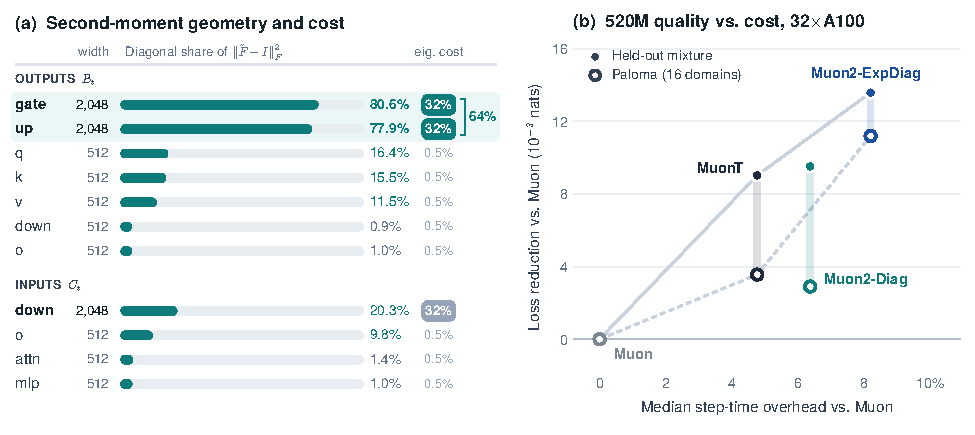
\includegraphics[width=\textwidth]{fig1_overview.pdf}
  \caption{\textbf{\mname{Muon2-ExpDiag} allocates dense output preconditioning where cross-channel geometry concentrates.}
  \textbf{(a)} Diagonal and off-diagonal shares of anisotropy across all 11 block second moments (130M, \mname{Muon} trajectory, step 2,500; 32-layer medians of $\mathrm{DiagAniso}$ in \cref{eq:diag_aniso} and $1-\mathrm{DiagAniso}$). The split shows where departure from isotropy lies in the coordinate basis rather than its total magnitude. The cost column gives each moment's share of nominal two-sided dense eigendecomposition work; teal marks the two expanded outputs (\texttt{gate,up}) that \mname{Muon2-ExpDiag} diagonalizes, which account for 96.2\% of output-side cubic work while carrying mostly diagonal anisotropy. The equally wide \texttt{down} input remains cross-channel correlated and stays dense.
  \textbf{(b)} Final held-out mixture and 16-domain Paloma loss reductions versus \mname{Muon} at 520M against median step-time overhead on 32 A100 GPUs (one seed). \mname{Muon2-ExpDiag} extends \mname{MuonT}'s quality gain with modest median overhead, whereas all-diagonal output scaling (\mname{Muon2-Diag}) adds almost no held-out gain and falls behind \mname{MuonT} on Paloma.}
  \label{fig:overview}
\end{figure}

\paragraph{Why Transformer geometry favors asymmetric compute.}
Auditing second-moment trajectories across all 32 Transformer blocks explains why \mname{Muon2-ExpDiag} allocates compute unevenly across roles and sides (\Cref{sec:diagnosis}; \Cref{fig:overview}(a)). On the gated \texttt{gate} and \texttt{up} expansion outputs, unequal coordinate second moments account for 78--91\% of total departure from isotropy, so diagonal scaling closely tracks the dense inverse root right where cubic cost concentrates. The hidden-width residual writers (\texttt{o} and \texttt{down}) show the opposite geometry: their coordinate second moments are nearly uniform, and over 99\% of their anisotropy lies in cross-channel correlations where diagonal scaling acts nearly as identity. Matrix width alone does not explain this split, because the equally wide \texttt{down} \emph{input} remains strongly correlated across channels and therefore stays dense. Over time, leading cotangent eigenspaces also rotate roughly an order of magnitude faster than RMSNormed inputs, causing cached-eigenbasis solvers to trigger frequent exact eigendecompositions that would stall synchronous updates.

\paragraph{Pretraining gains across seeds, horizon, and width.}
Across pretraining benchmarks (\Cref{sec:scaling}), \mname{Muon2-ExpDiag} improves consistently over tuned \mname{MuonT} at their shared full-budget learning rate. It lowers final held-out mixture loss by $0.0035\pm0.0017$ nats across three fresh paired seeds at 130M, by $0.0040$ nats when training four times longer (10.74B tokens), and by $0.0046$ nats under width transfer to 520M, where it also improves every one of the 16 out-of-distribution Paloma domains (\Cref{fig:overview}(b)). Across these three regimes, \mname{Muon2-ExpDiag} extends \mname{MuonT}'s held-out improvement over \mname{Muon} by 29--51\%.

\paragraph{Controls, weight decay, and update mechanism.}
Matched execution-path identity controls (\mname{Null-Ctrl}), full-budget learning-rate brackets, factor-placement ablations, and controlled comparisons with recent two-sided polar baselines (\mname{GO-MUON}, \mname{Mousse}) verify that these gains come from dense hidden-width output factors around the polar map rather than numerical drift or learning-rate mistuning (\Cref{sec:controls_ablations}). A multi-seed regularizer study further shows that keeping right-only weight decay ($W\hat R^2$) outperforms both isotropic ($W$) and two-sided ($\hat L^2 W\hat R^2$) decay across held-out, C4, and Paloma evaluations. On saved checkpoints, counterfactual probes and multi-checkpoint audits show that dense output factors rotate residual updates without inflating step norms and lower leading cotangent-subspace drift by 17--21\% relative to \mname{Muon} (\Cref{sec:mechanism_cost}).

\paragraph{Scope and runtime cost.}
Our experiments study pre-RMSNorm SwiGLU Transformers up to 537M non-embedding parameters. Relative to \mname{Muon}, expansion-output diagonalization and one-step lag cut median step-time overhead from 23.3\% (\mname{Muon2-Dense}) to 6.8\% at 130M and 8.2\% at 520M (5.3\% and 3.3\% above \mname{MuonT}), while periodic eigenbasis repairs leave mean overheads of 10.7\% and 17.0\% (8.9\% and 11.4\% above \mname{MuonT}). These results establish a fixed-token quality improvement at a modest remaining throughput cost; because the 80-TPP and 520M runs each use a single seed, multi-seed runs at larger scales are a natural next step.

\section{The WT-MLP-Lag optimizer}
\label{sec:method}

\mname{WT-MLP-Lag} extends input-whitened \mname{MuonT} into a practical two-sided polar optimizer through two co-designed choices: width-thresholded output preconditioning—retaining dense spectral factors on hidden-width outputs while diagonalizing expanded MLP outputs—and a one-update asynchronous lag that moves post-backward output processing off the critical path.

\subsection{Two-sided preconditioned Muon update}
\label{sec:operator}

We consider pre-RMSNorm SwiGLU Transformer blocks with hidden width $\dm$ and MLP expansion width $\dff=4\dm$. Each block contains seven 2D linear projections $y=W_{p,t}x$ with weight matrix $W_{p,t}\in\R^{m_p\times n_p}$: four square attention projections (\texttt{q,k,v,o} of shape $\dm\times\dm$), two tall expansion projections (\texttt{gate,up} of shape $\dff\times\dm$), and one wide contraction projection (\texttt{down} of shape $\dm\times\dff$). Given the globally averaged stochastic gradient $G_{p,t}\in\R^{m_p\times n_p}$, we maintain Nesterov momentum
\begin{equation}
 M_{p,t}=\mu M_{p,t-1}+G_{p,t},\qquad U_{p,t}=G_{p,t}+\mu M_{p,t},\qquad\mu=0.95,
 \label{eq:momentum}
\end{equation}
initialized at $M_{p,-1}=0$, and let $\Nten$ denote the ten-step mixed-precision Newton--Schulz polar map specified in \Cref{app:appendix_math}.

During forward and backward passes over $N_t$ sampled token positions $j$, each projection observes input activations $x_{p,t,j}\in\R^{n_p}$ and backpropagated output cotangents $\delta_{p,t,j}=\partial\ell/\partial y_{p,t,j}\in\R^{m_p}$. We track exponential moving averages of their uncentered second moments:
\begin{align}
 C_{g(p),t}&=\beta C_{g(p),t-1}+(1-\beta)N_t^{-1}\sum_jx_{p,t,j}x_{p,t,j}^{\Tr},\nonumber\\
 B_{p,t}&=\beta B_{p,t-1}+(1-\beta)N_t^{-1}\sum_j\delta_{p,t,j}\delta_{p,t,j}^{\Tr},
 \qquad \beta=0.938,
 \label{eq:moments}
\end{align}
corresponding to an effective horizon of $(1-\beta)^{-1}\approx 16$ updates. Moment sharing is inherently asymmetric between the two sides: because \texttt{q,k,v} share the pre-attention input and \texttt{gate,up} share the pre-MLP input, $g(p)$ collapses forward statistics to four input moments per block (three at width $\dm$ and \texttt{down} at width $\dff$), whereas distinct backward cotangents require seven separate output moments per block (five at width $\dm$ and \texttt{gate,up} at width $\dff$). To remove overall layerwise scale before forming inverse roots, any positive-trace moment $F\in\R^{d\times d}$ is trace-normalized and damped:
\begin{equation}
 \tilde F=\frac{dF}{\tr(F)},\qquad A_d(F)=\tilde F+\epsilon I_d,\qquad\epsilon=10^{-3}.
 \label{eq:trace_norm}
\end{equation}

Using right (input) inner and outer factors $(R_{p,t},\hat R_{p,t})$ built from $C_{g(p),t}$ and left (output) inner and outer factors $(L_{p,t-\tau},\hat L_{p,t-\tau})$ built from $B_{p,t-\tau}$ at staleness lag $\tau\in\{0,1\}$, we update each 2D projection via
\begin{align}
 D_{p,t}&=\hat L_{p,t-\tau}\,\Nten\!\left(L_{p,t-\tau}U_{p,t}R_{p,t}\right)\hat R_{p,t},\nonumber\\
 W_{p,t+1}&=W_{p,t}-\eta_t\left(s_{m_p,n_p}D_{p,t}+\lambda W_{p,t}\hat R_{p,t}^2\right),
 \label{eq:update}
\end{align}
with aspect-ratio scale $s_{m,n}=\sqrt{\max(1,m/n)}$, decoupled weight decay $\lambda=0.1$, and auxiliary AdamW on embeddings, RMSNorm gains, and the untied output head. Setting all four factors to identity recovers \mname{Muon}; setting $L=\hat L=I$ recovers \mname{MuonT}. Here $W_{p,t}\hat R_{p,t}^2$ is \mname{MuonT}'s metric-shaped weight decay from the right reparameterization $W=\widetilde W\hat R$ (\Cref{app:weight_decay}); \Cref{app:left_decay_asymmetry} derives the two-sided counterpart $\hat L^2 W\hat R^2$ and analyzes the structural and experimental-control motivations for retaining one-sided $W\hat R^2$.

\subsection{Width-thresholded factor assignment}
\label{sec:factor_assignment}

Following \mname{MuonT}'s decoupled exponent split, each preconditioned side pairs a $-1/2$ inner whitening factor before $\Nten$ with a unit-RMS $-1/8$ outer scaling factor after $\Nten$, instantiated in either dense spectral ($\mathsf{Dense}$) or coordinate diagonal ($\mathsf{Diag}$) form:
\begin{align}
 R&=A_n(C)^{-1/2},&\hat R&=\unitrms\!\left(A_n(C)^{-1/8}\right),\nonumber\\
 L^{\mathsf{Dense}}&=A_m(B)^{-1/2},&\hat L^{\mathsf{Dense}}&=\unitrms\!\left(A_m(B)^{-1/8}\right),
 \label{eq:dense_roots}\\
 L^{\mathsf{Diag}}&=\Diag(a^{-1/2}),&\hat L^{\mathsf{Diag}}&=\unitrms\!\left(\Diag(a^{-1/8})\right),
 \label{eq:diag_roots}
\end{align}
where $a=m\diag(B)/\tr(B)+\epsilon\mathbf1$ and $\unitrms(X)=\sqrt d\,X/\|X\|_F$ for a $d\times d$ matrix. Scaling outer factors to unit RMS prevents trivial step-size inflation from matrix trace changes; we verify empirical update norms directly on saved checkpoints in \Cref{sec:mechanism}.

\begin{table}[!htb]\centering\small
\setlength{\tabcolsep}{4.0pt}
\caption{\textbf{Factor assignment and nominal output $O(d^3)$ share across core methods.} Dense and Diag denote the $(-1/2,-1/8)$ factor pairs in \Cref{eq:dense_roots,eq:diag_roots}. Splitting both sides by projection role and width ($\dm$ versus $\dff=4\dm$) highlights the structural asymmetry: Muon2-ExpDiag retains dense factors on the $\dff$-wide \texttt{down} input while diagonalizing the two $\dff$-wide gated MLP expansion outputs (\texttt{gate,up}). Fine-grained placement ablations appear in \Cref{tab:ablations}.}\label{tab:taxonomy}
\begin{tabularx}{\textwidth}{@{}>{\raggedright\arraybackslash}Xcccccr@{}}
\toprule
& \multicolumn{2}{c}{Input factors ($R,\hat R$)} & \multicolumn{2}{c}{Output factors ($L,\hat L$)} & & \\
\cmidrule(lr){2-3}\cmidrule(lr){4-5}
Method & $\dm$ (\texttt{attn,o,mlp}) & $\dff$ (\texttt{down}) & $\dm$ (\texttt{q,k,v,o,down}) & $\dff$ (\texttt{gate,up}) & Lag $\tau$ & Out $O(d^3)$ \\
\midrule
Muon & $I$ & $I$ & $I$ & $I$ & --- & 0\% \\
MuonT & Dense & Dense & $I$ & $I$ & --- & 0\% \\
Muon2-Diag & Dense & Dense & Diag & Diag & 0 & 0\% \\
Abl-SymDiag & Dense & Diag & Dense & Diag & 1 & 3.8\% \\
Muon2-ExpDiag (sync) & Dense & Dense & Dense & Diag & 0 & 3.8\% \\
\rowcolor{rowtint}[0pt][0pt]\textbf{Muon2-ExpDiag} & \textbf{Dense} & \textbf{Dense} & \textbf{Dense} & \textbf{Diag} & \textbf{1} & \textbf{3.8\%} \\
Muon2-Dense & Dense & Dense & Dense & Dense & 0 & 100\% \\
Null-Ctrl & Dense & Dense & $I$ (after solve) & $I$ (after solve) & 0 & 3.8\% \\
\bottomrule\end{tabularx}
\end{table}


\mname{WT-MLP-Lag} assigns these operators asymmetrically by side and projection width (\Cref{tab:taxonomy}, \Cref{fig:method_pipeline}(a)):
\begin{itemize}
 \item \textbf{All inputs ($\dm$ and $\dff$):} Dense spectral factors $(R,\hat R)$ on all four input moments, including the $\dff$-wide \texttt{down} input, exactly as in \mname{MuonT}.
 \item \textbf{Hidden-width outputs ($\dm$: \texttt{q,k,v,o,down}):} Dense spectral factors $(L^{\mathsf{Dense}},\hat L^{\mathsf{Dense}})$ to capture cross-channel cotangent correlations, held for one update ($\tau=1$).
 \item \textbf{Expansion-width outputs ($\dff$: \texttt{gate,up}):} Exact per-step diagonal factors $(L^{\mathsf{Diag}},\hat L^{\mathsf{Diag}})$ computed inline without forming $\dff\times\dff$ Gram matrices or eigendecompositions.
\end{itemize}
With five $\dm$-wide and two $\dff$-wide output moments per block, the two expansion outputs account for
\begin{equation}
 \frac{2(4\dm)^3}{5\dm^3+2(4\dm)^3}=96.2\%
 \label{eq:cubic_share}
\end{equation}
of nominal dense output $O(d^3)$ eigendecomposition work and 86.5\% of output Gram storage. Width thresholding therefore eliminates nearly all cubic output-side work while retaining dense spectral conditioning on every hidden-width projection.

\begin{figure}[t]
 \centering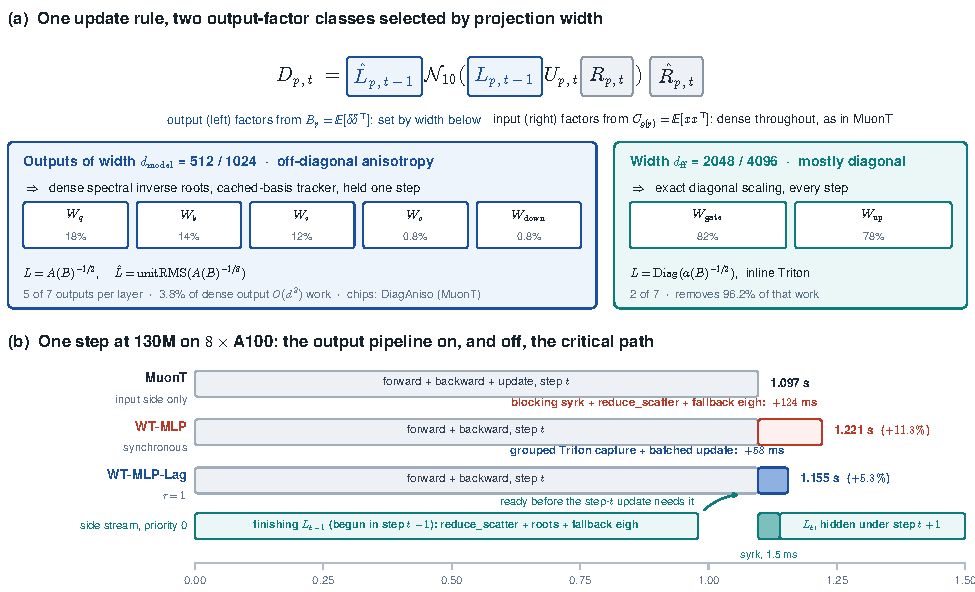
\includegraphics[width=\textwidth]{fig3_method_pipeline.pdf}
 \caption{\textbf{Factor assignment and asynchronous execution pipeline of \mname{WT-MLP-Lag}.}
 \textbf{(a)} Update rule and width-thresholded output classes: dense spectral factors on the five $\dm$-wide outputs (\texttt{q,k,v,o,down}), inline exact diagonal scaling on the two $\dff$-wide expansion outputs (\texttt{gate,up}), and dense input factors throughout. Chip percentages preview each output moment's diagonal share of anisotropy along \mname{MuonT} (\Cref{sec:diagnosis}).
 \textbf{(b)} Single-step execution timeline at 130M scaled to measured eight-A100 medians (\Cref{tab:bench19}). Synchronous \mname{WT-MLP} stalls at the step boundary waiting for output reductions and fallback eigensolves; with a one-update lag ($\tau=1$), \mname{WT-MLP-Lag} applies ready factors immediately while computing new output roots alongside step $t+1$.}
 \label{fig:method_pipeline}
\end{figure}

The inner and outer output factors play distinct geometric roles around $\Nten$. Inner whitening ($L$) changes which output directions dominate the pre-polar singular frame; even when polar orthogonalization normalizes singular values, non-commuting left whitening rotates the resulting orthogonal row frame (\Cref{sec:mechanism}). Post-polar scaling ($\hat L$) subsequently adjusts how much update magnitude is allocated along each output eigendirection. Inherited from \mname{MuonT}, the gentler $-1/8$ outer exponent avoids over-amplifying low-variance cotangent modes and is tested against outer-only and steeper-exponent alternatives in \Cref{sec:controls_ablations}.

\subsection{Asynchronous one-step-lagged execution}
\label{sec:systems}

Forward activations materialize during the forward pass, allowing \mname{MuonT} to overlap input-factor updates with backpropagation. Output cotangents, by contrast, finish arriving only at the end of backward right before the parameter update. To remove output moment reduction and root solving from this critical boundary, \mname{WT-MLP-Lag} sets $\tau=1$ (\Cref{fig:method_pipeline}(b)): step $t$'s parameter update immediately consumes $(L_{t-1},\hat L_{t-1})$ (initialized to identity at $t=0$) together with current input factors, while a priority-0 CUDA side stream contracts, reduce-scatters, and roots step $t$'s captured output statistics underneath step $t+1$'s forward and backward passes. The next update waits only if those background kernels have not yet finished. Although a one-step lag is small relative to the 16-update EMA horizon, we verify directly in \Cref{sec:ablations} that $\tau=1$ preserves nearly all of synchronous \mname{WT-MLP}'s loss improvement.

Three kernel-level optimizations keep statistics capture and dense products lightweight. First, grouped Triton backward hooks capture cotangents at shared autograd nodes; for diagonal \texttt{gate,up} outputs, an inline reduction accumulates squared cotangents directly into FP32 vectors, while dense $\dm$-wide outputs use chunked row buffers that flush partial Grams during gradient accumulation so memory does not grow with microbatch count (permitting larger per-GPU microbatches at 520M). Second, because cotangent eigenspaces rotate rapidly (\Cref{sec:drift_cost}), the cached-eigenbasis root tracker uses GPU-resident residual checks and batched exact fallback eigendecompositions to avoid host synchronization. Third, matching-shape projections share batched update kernels, grouped projections reuse input-factor products, and dense pre- and post-polar matrix multiplications use the FP16-split Tensor-Core arithmetic detailed in \Cref{app:appendix_math}.

\section{Why width thresholding and overlap fit Transformer geometry}
\label{sec:diagnosis}

\mname{WT-MLP-Lag} rests on two empirical hypotheses about Transformer pretraining: that the expensive $\dff$-wide expansion outputs are well approximated by diagonal scaling whereas hidden-width outputs—and $\dff$-wide inputs—require dense cross-channel factors, and that output eigenspaces drift too rapidly for synchronous cached-basis solvers. We test both hypotheses directly by auditing all 11 input and output second moments across all 32 blocks on \mname{Muon}, \mname{MuonT}, and \mname{WT-MLP-Lag} trajectories at 130M ($\dm=512,\dff=2{,}048$). Both patterns hold across all three optimizers, indicating that they reflect block architecture rather than a single optimizer's trajectory.

\subsection{Auditing coordinate and cross-channel moments}
\label{sec:diagnosis_setup}

For any trace-normalized second moment $\tilde F=dF/\tr(F)$ from \cref{eq:trace_norm}, we decompose its squared Frobenius departure from identity into orthogonal coordinate (diagonal) and cross-channel (off-diagonal) components:
\begin{equation}
 \begin{aligned}
 E_{\rm diag}&=\sum_i(\tilde F_{ii}-1)^2,\qquad E_{\rm off}=\sum_{i\ne j}\tilde F_{ij}^2,\\
 \mathrm{DiagAniso}(F)&=\frac{E_{\rm diag}}{E_{\rm diag}+E_{\rm off}}
 =\frac{\|\diag(\tilde F)-\mathbf1\|_2^2}{\|\tilde F-I_d\|_F^2},\\
 \text{Off-diagonal share}&=\frac{E_{\rm off}}{E_{\rm diag}+E_{\rm off}}
 =1-\mathrm{DiagAniso}(F),
 \end{aligned}
 \label{eq:diag_aniso}
\end{equation}
where $E_{\rm diag}+E_{\rm off}=\|\tilde F-I_d\|_F^2$ identically. Replacing identity with the best diagonal approximation removes exactly $E_{\rm diag}$ of squared Frobenius error, so $\mathrm{DiagAniso}(F)$ measures the fraction of moment anisotropy aligned with the coordinate axes. Because $\mathrm{DiagAniso}(F)$ is a relative share rather than a magnitude—a non-isotropic diagonal matrix has share one even near identity—we pair it in \Cref{tab:diagnosis_summary} with off-diagonal uncentered correlation RMS ($\rho_{\rm rms}$), direct inverse-root fidelity ($R^2$ between $L^{\mathsf{Diag}}$ and $L^{\mathsf{Dense}}$ relative to identity in \cref{eq:r2_root}), and 250-step top-16 eigenspace drift ($\mathrm{Drift}_{16}$ in \cref{eq:subspace_drift}). Complete metric derivations, replay checks, and the full 352-matrix ledger appear in \Cref{app:appendix_mech,tab:diagnosis}.

\begin{figure}[t]
 \centering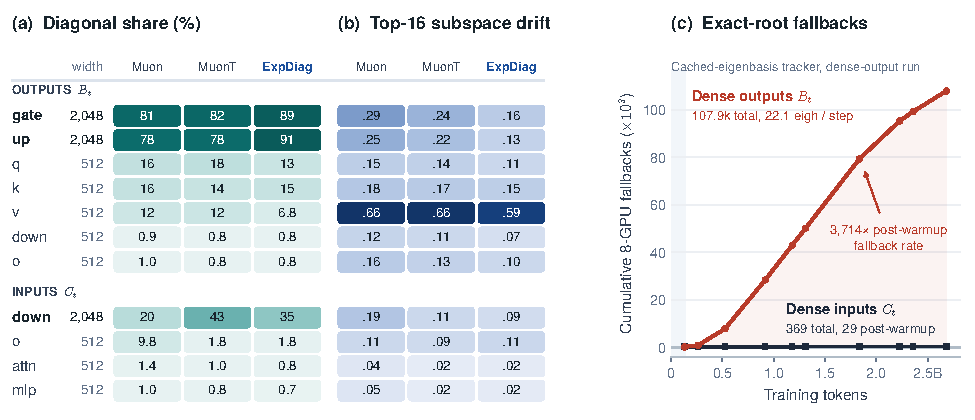
\includegraphics[width=\textwidth]{fig2_structural_audit.pdf}
 \caption{\textbf{Projection role separates moment geometry and drift across \mname{Muon}, \mname{MuonT}, and \mname{WT-MLP-Lag}.}
 \textbf{(a)} 32-layer median diagonal anisotropy share ($\mathrm{DiagAniso}$ in \cref{eq:diag_aniso}) at step 2,500 (130M); its complement is the off-diagonal share. Expanded SwiGLU outputs (\texttt{gate,up}) are predominantly diagonal across all three optimizers, whereas residual writers (\texttt{o,down}) carry less than 1\% of anisotropy on the diagonal.
 \textbf{(b)} 32-layer mean top-16 subspace drift from steps 2,250 to 2,500 (defined in \cref{eq:subspace_drift}; $0$ denotes identical subspaces and $1$ orthogonal subspaces).
 \textbf{(c)} Cumulative exact-eigendecomposition fallbacks across eight GPUs in the dense-output diagnostic run: dense outputs trigger 22.1 exact repairs per step versus 29 post-warmup fallbacks in total for dense inputs.}
 \label{fig:structural_audit}
\end{figure}

\begin{table}[tbp]\centering\footnotesize
\setlength{\tabcolsep}{5.8pt}
\caption{\textbf{Moment geometry and subspace drift by projection role at 130M.} Static columns report 32-layer medians on the Muon baseline trajectory at step 2,500 (matching \Cref{fig:overview}(a)). For diagonal anisotropy share (DA), parentheses give the range of these medians across Muon, MuonT, and Muon2-ExpDiag. $\rho_{\rm rms}$ is the RMS of off-diagonal uncentered correlations; root $R^2$ compares diagonal and dense inverse roots. Drift compares the subspaces at steps 2,250 and 2,500, averaged over 32 layers for each trajectory (ExpDiag denotes Muon2-ExpDiag). ExpDiag uses a resumed trajectory; uninterrupted-checkpoint comparisons are reported in \Cref{sec:output_drift}. Tinted expansion outputs account for 96.2\% of nominal dense output eigendecomposition work.}\label{tab:diagnosis_summary}
\begin{tabularx}{\textwidth}{@{}>{\raggedright\arraybackslash}Xrrrrrrr@{}}
\toprule
& & & \multicolumn{2}{c}{Diagonal fidelity} & \multicolumn{3}{c}{250-step $\mathrm{Drift}_{16}$} \\
\cmidrule(lr){4-5}\cmidrule(lr){6-8}
Moment & $d$ & $\rho_{\rm rms}$ & DA (\%, 3-traj) & Root $R^2$ (\%) & Muon & MuonT & ExpDiag \\
\midrule
\addlinespace[2pt]\multicolumn{8}{@{}l}{\textit{Input activation moments $C_t=\E[xx^{\Tr}]$ (4 per block)}}\\
attention & 512 & 0.147 & 1.4 (0.8--1.4) & 8.2 & 0.041 & 0.021 & 0.023 \\
o & 512 & 0.097 & 9.8 (1.8--9.8) & 30.1 & 0.107 & 0.094 & 0.108 \\
MLP & 512 & 0.141 & 1.0 (0.7--1.0) & 4.9 & 0.046 & 0.021 & 0.025 \\
down & 2,048 & 0.028 & 20.3 (20.3--43.4) & 91.3 & 0.186 & 0.106 & 0.087 \\
\addlinespace[5pt]\multicolumn{8}{@{}l}{\textit{Output cotangent moments $B_t=\E[\delta\delta^{\Tr}]$ (7 per block)}}\\
q & 512 & 0.061 & 16.4 (13.3--18.0) & 64.8 & 0.150 & 0.140 & 0.110 \\
k & 512 & 0.075 & 15.5 (14.4--15.5) & 77.6 & 0.178 & 0.165 & 0.147 \\
v & 512 & 0.060 & 11.5 (6.8--12.2) & 38.6 & 0.664 & 0.662 & 0.586 \\
\addlinespace[2.5pt]
o (res.) & 512 & 0.031 & 1.0 (0.8--1.0) & 3.6 & 0.164 & 0.134 & 0.103 \\
down (res.) & 512 & 0.032 & 0.9 (0.8--0.9) & 2.3 & 0.123 & 0.107 & 0.072 \\
\addlinespace[2.5pt]
\rowcolor{rowtint}[0pt][0pt]gate (exp.) & 2,048 & 0.005 & 80.6 (80.6--89.5) & 98.8 & 0.292 & 0.240 & 0.159 \\
\rowcolor{rowtint}[0pt][0pt]up (exp.) & 2,048 & 0.007 & 77.9 (77.9--90.8) & 98.2 & 0.251 & 0.215 & 0.130 \\
\bottomrule\end{tabularx}
\end{table}


\subsection{Dense correlations at hidden width; coordinate scaling at expansion width}
\label{sec:dichotomy}

\Cref{fig:structural_audit}(a) and \Cref{tab:diagnosis_summary} show a sharp separation by projection role. On the $\dff$-wide \texttt{gate} and \texttt{up} outputs, coordinate energy accounts for 78--91\% of total anisotropy across all three trajectories, off-diagonal correlations sit near $\rho_{\rm rms}=0.005\text{--}0.008$, and diagonal inverse roots capture 76--99\% of squared Frobenius distance to the dense inverse root. Structurally, these cotangents backpropagate through elementwise SwiGLU gates, multiplying the upstream gradient vector coordinatewise by token-dependent forward gating factors. The weak cross-channel correlations are consistent with this elementwise gating suppressing shared cross-channel output structure (though our empirical audit does not claim a general decorrelation theorem). Approximating these two moments with $L^{\mathsf{Diag}}$ and $\hat L^{\mathsf{Diag}}$ therefore preserves most of their conditioning while removing 96.2\% of nominal cubic output work in \cref{eq:cubic_share}.

The hidden-width residual writers \texttt{o} and \texttt{down} exhibit the opposite geometry. Unequal coordinate second moments account for only 0.8--1.0\% of their anisotropy, and diagonal inverse roots reduce squared error relative to identity by less than 4\% ($R^2=1.2\text{--}3.6\%$). Purely diagonal output preconditioning (\mname{OD-All}) thus acts nearly as identity on the projections writing back into the residual stream. The attention-internal outputs (\texttt{q,k,v}) fall between these regimes (7--18\% diagonal anisotropy; 20--79\% root $R^2$), carrying substantial off-diagonal structure at affordable width $\dm$ and motivating \mname{WT-MLP-Lag}'s retention of dense spectral roots on all five $\dm$-wide outputs.

Crucially, matrix width alone does not justify diagonalization on both sides. The equally wide $\dff=2{,}048$ \texttt{down} \emph{input} retains 57--80\% of its anisotropy off the diagonal ($\mathrm{DiagAniso}=20\text{--}43\%$, $\rho_{\rm rms}\approx 0.035$), as post-SwiGLU activations remain coupled through the shared $\dm$-dimensional token representation. This input--output asymmetry explains why \mname{WT-MLP-Lag} thresholds only the output side while keeping \texttt{in:down} dense—a choice confirmed empirically when symmetric $\dff$ diagonalization (\mname{WT-Sym-Lag}) sacrifices most of the loss gain in \Cref{sec:ablations}.

\subsection{Fast cotangent subspace drift requires asynchronous repairs}
\label{sec:drift_cost}

Even after removing $\dff\times\dff$ output eigendecompositions, the five $\dm$-wide output moments behave very differently over time from forward input moments (\Cref{fig:structural_audit}(b,c)). Along \mname{MuonT}, 250-step top-16 subspace drift is roughly $0.021$ on RMSNormed attention and MLP inputs, compared with $0.107\text{--}0.662$ across output cotangents. Consequently, a cached-eigenbasis root tracker that needs only 29 exact eigendecomposition fallbacks after warmup across all dense inputs triggers roughly 22 exact fallbacks \emph{per step} (107.9k cumulative across eight GPUs) when applied to dense outputs. (\Cref{sec:output_drift} extends this single-interval audit to uninterrupted checkpoints across full 130M and 520M training trajectories.)

Because cotangents arrive at the end of backpropagation, running distributed Gram reductions and frequent fallback eigensolves synchronously stalls every step boundary (\Cref{fig:method_pipeline}(b)). Pairing width thresholding with the $\tau=1$ asynchronous side-stream schedule in \Cref{sec:systems} addresses both halves of the cost bottleneck: mathematical approximation removes the $\dff^3$ solves, and one-step overlap hides most of the remaining $\dm^3$ repairs beneath the next forward and backward pass.

\section{Pretraining experiments and scaling}
\label{sec:scaling}

We evaluate \mname{WT-MLP-Lag} against unpreconditioned \mname{Muon}, tuned input-only \mname{MuonT}, and all-diagonal output preconditioning (\mname{OD-All}) across three pretraining regimes: multi-seed confirmation at 130M (20 tokens per non-embedding parameter, TPP), fourfold horizon scaling at 130M (80 TPP, 10.74B tokens), and width transfer to 520M (20 TPP, 10.74B tokens). Across all three regimes, \mname{WT-MLP-Lag} lowers final held-out loss relative to \mname{MuonT}, extending \mname{MuonT}'s held-out gain over \mname{Muon}—$(\mathcal L_{\rm MuonT}-\mathcal L_{\rm WT})/(\mathcal L_{\rm Muon}-\mathcal L_{\rm MuonT})$, with denominators $0.0119$, $0.0103$, and $0.0090$ nats—by 29--51\%.

\subsection{Experimental setup}
\label{sec:testbed}

We train 32-layer, pre-RMSNorm SwiGLU Transformers on a 25.4B-token mixture of DCLM, StarCoderData, and Proof-Pile-2 in the Marin PyTorch suite~\citep{mohamadi2026toner}, using the Llama-3.1 vocabulary of 128,256 tokens, sequence length 4,096, document-isolated causal attention, and NVIDIA A100-40GB GPUs. Within every seed, all optimizer arms share parameter initialization and minibatch data ordering. The labels 130M and 520M denote models with approximately 134M ($\dm=512,\dff=2{,}048$) and 537M ($\dm=1{,}024,\dff=4{,}096$) non-embedding parameters (\Cref{tab:regimes}).

\suppressfloats[t]
\begin{table}[tbp]\centering\small
\setlength{\tabcolsep}{5.8pt}
\caption{\textbf{Pretraining regimes.} Params counts non-embedding parameters; TPP is tokens per non-embedding parameter. Fresh-seed confirmation uses seeds 1--3 after learning-rate selection and execution-path checks on seed 0.}\label{tab:regimes}
\begin{tabularx}{\textwidth}{@{}>{\raggedright\arraybackslash}Xrrrrrc@{}}
\toprule
Regime & Params & $\dm$ / $\dff$ & Tokens (TPP) & Batch / Steps & GPUs & Seeds \\
\midrule
130M controls \& LR bracket & 134M & 512 / 2,048 & 2.68B (20) & 0.5M / 5,120 & 8$\times$A100 & 0 \\
130M confirmation & 134M & 512 / 2,048 & 2.68B (20) & 0.5M / 5,120 & 8$\times$A100 & 1, 2, 3 \\
130M longer training & 134M & 512 / 2,048 & 10.74B (80) & 0.5M / 20,480 & 8$\times$A100 & 0 \\
520M width transfer & 537M & 1,024 / 4,096 & 10.74B (20) & 1.0M / 10,240 & 32$\times$A100 & 0 \\
\bottomrule\end{tabularx}
\end{table}


We evaluate completed models on held-out training-mixture cross-entropy $\Lsel$, C4 cross-entropy $\Lc$, and the unweighted macro average across 16 out-of-distribution Paloma domains $\Lpal$. To check whether gains persist throughout late training rather than appearing only at schedule end, we also report paired means over the 11 second-half evaluation checkpoints (Late-11; correlated trajectory observations rather than independent seeds). Differences are reported in millinats ($1\text{ mnat}=10^{-3}\text{ nats}$, negative favoring the row method). Because short-schedule proxy sweeps select overly aggressive learning rates that degrade full-budget runs (\Cref{sec:falsification}), we sweep $\eta\in\{0.01131,0.016,0.02263,0.032\}$ at the full 2.68B-token budget on seed 0, where all four core methods share the same strict interior optimum $\eta^*=0.0160$.

\begin{table}[!htb]\centering\small
\setlength{\tabcolsep}{1.5pt}
\caption{\textbf{Confirmatory and scaling results across fresh seeds, longer horizon, and greater width.} Held-out reports final cross-entropy $\Lsel$ in nats; all $\Delta$ columns report differences from same-regime Muon in millinats (negative favors the row method). MuonT applies input preconditioning only, so the gap between the MuonT and Muon2-ExpDiag rows isolates the output-side contribution. Late-11 averages the 11 second-half checkpoints; Wins counts the 16 Paloma domains improved over Muon. All four methods share their verified seed-0 optimum within each regime ($\eta^*=0.01600$ at 130M and 520M 20 TPP, and $0.01600\times4^{-0.3}=0.01056$ at 130M 80 TPP). Complete absolute losses and $\eta=0.02263$ replicates appear in \Cref{tab:absolute_results,tab:seeds}.}\label{tab:main_scaling}
\begin{tabularx}{\textwidth}{@{}>{\raggedright\arraybackslash}Xrrrrrrr@{}}
\toprule
& & (nats) & \multicolumn{4}{c}{Differences from Muon (millinats, $\downarrow$)} & OOD \\
\cmidrule(lr){4-7}
Method & LR $\eta$ & Held-out & $\Delta$ Held-out & Late-11 $\Delta$ & $\Delta$ C4 & $\Delta$ Paloma & Wins \\
\midrule
\addlinespace[2pt]\multicolumn{8}{@{}l}{\textit{130M confirmation: 20 TPP, 2.68B tokens, fresh seeds 1--3 (matched $\eta^*=0.0160$, paired mean $\pm$ SD)}}\\
Muon & 0.01600 & 3.2035 & $+0.00$ & $+0.00$ & $+0.00$ & $+0.00$ & --- \\
MuonT & 0.01600 & 3.1916 & $-11.91\pm1.40$ & $-23.26\pm2.07$ & $-11.79\pm0.98$ & $-11.49\pm4.18$ & 16/16 \\
Muon2-Diag & 0.01600 & 3.1919 & $-11.62\pm1.09$ & $-22.91\pm1.63$ & $-12.63\pm1.22$ & $-12.79\pm1.92$ & 16/16 \\
\rowcolor{rowtint}[0pt][0pt]\textbf{Muon2-ExpDiag} & 0.01600 & \textbf{3.1881} & $\mathbf{-15.41\pm2.18}$ & $\mathbf{-26.78\pm2.30}$ & $\mathbf{-15.64\pm1.80}$ & $\mathbf{-15.91\pm1.68}$ & \textbf{16/16} \\
\addlinespace[5pt]\multicolumn{8}{@{}l}{\textit{130M longer training: 80 TPP, 10.74B tokens, seed 0 (matched rate)}}\\
Muon & 0.01056 & 3.0778 & $+0.00$ & $+0.00$ & $+0.00$ & $+0.00$ & --- \\
MuonT & 0.01056 & 3.0675 & $-10.28$ & $-22.28$ & $-10.26$ & $-11.12$ & 15/16 \\
Muon2-Diag & 0.01056 & 3.0656 & $-12.19$ & $-23.85$ & $-12.82$ & $-13.71$ & 16/16 \\
\rowcolor{rowtint}[0pt][0pt]\textbf{Muon2-ExpDiag} & 0.01056 & \textbf{3.0636} & $\mathbf{-14.23}$ & $\mathbf{-26.82}$ & $\mathbf{-14.07}$ & $\mathbf{-16.78}$ & \textbf{16/16} \\
\addlinespace[5pt]\multicolumn{8}{@{}l}{\textit{520M width transfer: 20 TPP, 10.74B tokens, $\dm=1{,}024$, seed 0 (matched $\eta^*=0.0160$)}}\\
Muon & 0.01600 & 2.8528 & $+0.00$ & $+0.00$ & $+0.00$ & $+0.00$ & --- \\
MuonT & 0.01600 & 2.8438 & $-9.02$ & $-20.00$ & $-7.33$ & $-3.56$ & 15/16 \\
Muon2-Diag & 0.01600 & 2.8433 & $-9.52$ & $-21.97$ & $-9.52$ & $-2.90$ & 12/16 \\
\rowcolor{rowtint}[0pt][0pt]\textbf{Muon2-ExpDiag} & 0.01600 & \textbf{2.8392} & $\mathbf{-13.57}$ & $\mathbf{-24.68}$ & $\mathbf{-11.62}$ & $\mathbf{-11.19}$ & \textbf{16/16} \\
\bottomrule\end{tabularx}
\end{table}


\subsection{Multi-seed confirmation at 130M}
\label{sec:phase2}

On fresh 130M seeds 1--3 at the shared full-budget optimum $\eta^*=0.0160$, \mname{WT-MLP-Lag} outperforms both \mname{Muon} and \mname{MuonT} on every seed across held-out mixture, C4, Paloma macro loss, and Late-11 checkpoints (\Cref{tab:main_scaling}, \Cref{fig:scaling_traj}(a)). Relative to same-seed \mname{MuonT}, \mname{WT-MLP-Lag} lowers final held-out loss by $0.0035\pm0.0017$ nats (mean $\pm$ sample standard deviation across seeds), whereas purely diagonal \mname{OD-All} leaves held-out mixture loss essentially unchanged ($+0.0003\pm0.0004$ nats). Replicating both output methods on the same three seeds at the hotter grid point $\eta=0.02263$ preserves this separation ($0.0034\pm0.0015$ versus $0.0005\pm0.0005$ nats; \Cref{tab:absolute_results,tab:seeds}). Retaining cross-channel output correlations at hidden width—rather than coordinate scaling or learning-rate selection—therefore accounts for the 130M improvement.

The gain also holds when doubling the global batch size to 1M tokens: the checked 130M run improves over \mname{MuonT} by $0.0036$ nats on held-out mixture and $0.0040$ nats on C4 (a single-seed batch-size check rather than an additional multi-seed replication).

\subsection{Longer training at four times the token budget}
\label{sec:phase3}

Training the 130M model for 10.74B tokens (80 TPP) tests whether input-only \mname{MuonT} closes the gap given four times as much data. Following Marin's standard $T^{-0.3}$ token-horizon rule at fixed batch size~\citep{mohamadi2026toner}, we scale the shared 20-TPP optimum to $\eta=0.016\times4^{-0.3}=0.01056$: \mname{WT-MLP-Lag} finishes $0.0040$ nats lower than \mname{MuonT} on held-out mixture and remains ahead at every second-half checkpoint (\Cref{tab:main_scaling}, \Cref{fig:scaling_traj}(b)), while its out-of-distribution Paloma macro gain reaches $0.0057$ nats across all 16 domains (\Cref{fig:paloma}(a)). Scaling instead from the adjacent $\sqrt2$-step grid point $\eta=0.02263=0.016\sqrt2$ ($\eta=0.01493$, $\sqrt2\times$ higher) incurs a mid-training penalty and finishes worse on Paloma (\Cref{fig:scaling_traj}(b), \Cref{tab:absolute_results}), confirming that output preconditioning still requires horizon-appropriate learning rates.

\begin{figure}[t]
 \centering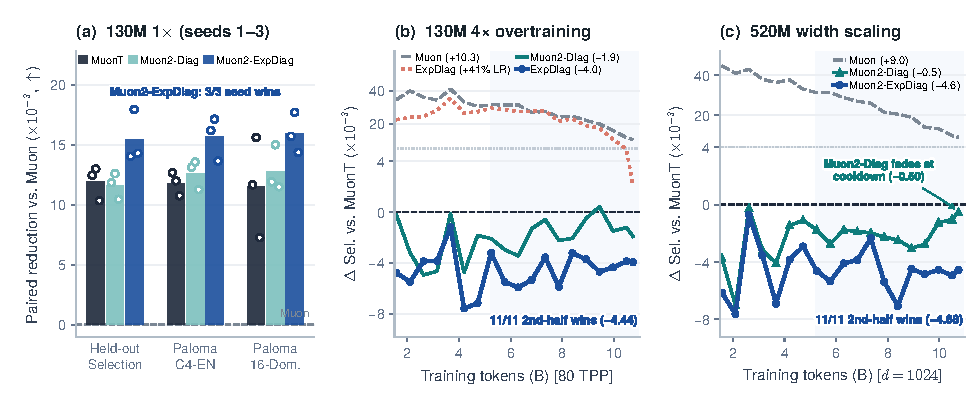
\includegraphics[width=\textwidth]{fig5_scaling_trajectories.pdf}
 \caption{\textbf{\mname{WT-MLP-Lag} improves over \mname{Muon} and \mname{MuonT} across fresh seeds, longer horizons, and greater width.}
 \textbf{(a)} Final loss reductions versus same-seed \mname{Muon} at 130M, 20 TPP; bars show three-seed means and open circles show individual seeds 1--3.
 \textbf{(b, c)} Held-out selection loss differences from \mname{MuonT} across 10.74B-token runs: 130M at 80 TPP and 520M at 20 TPP (one seed each; negative values favor the method). The hotter \mname{WT} curve in (b) illustrates horizon learning-rate sensitivity. Vertical axes compress the positive range above the dotted line.}
 \label{fig:scaling_traj}
\end{figure}

\subsection{Width transfer to 520M separates dense from all-diagonal outputs}
\label{sec:phase4}

Doubling model width to $\dm=1{,}024$ ($\dff=4{,}096$) cleanly separates width-thresholded dense outputs from purely diagonal outputs (\Cref{tab:main_scaling}, \Cref{fig:scaling_traj}(c)). Checking $\eta\in\{0.016,0.02263\}$ across all four methods at 520M selects the same shared optimum $\eta^*=0.016$ for every optimizer (\Cref{tab:absolute_results}). At this matched rate without output-side retuning, \mname{WT-MLP-Lag} lowers final held-out loss by $0.0046$ nats below \mname{MuonT} ($0.0043$ nats on C4) and leads at all 11 second-half checkpoints, whereas \mname{OD-All} gains only $0.0005$ nats on held-out mixture as its mid-training advantage fades during cooldown (at the hotter $\eta=0.02263$ rate, \mname{WT-MLP-Lag} still leads \mname{MuonT} by $0.0028$ nats while \mname{OD-All} finishes $0.0006$ nats worse; \Cref{tab:absolute_results}).

Per-domain evaluation on Paloma sharpens this contrast (\Cref{fig:paloma}(b), \Cref{tab:paloma_full}): at $\eta^*=0.016$, \mname{WT-MLP-Lag} improves over \mname{MuonT} in all 16 domains ($-7.63$ mnats macro mean), whereas \mname{OD-All} improves in 12 domains, regresses on four, and finishes worse than \mname{MuonT} overall ($+0.66$ mnats). Because Paloma domains share training and evaluation influences, win counts summarize out-of-distribution breadth within a run rather than independent replications, and two model widths do not establish an asymptotic scaling law.

\begin{figure}[t]
 \centering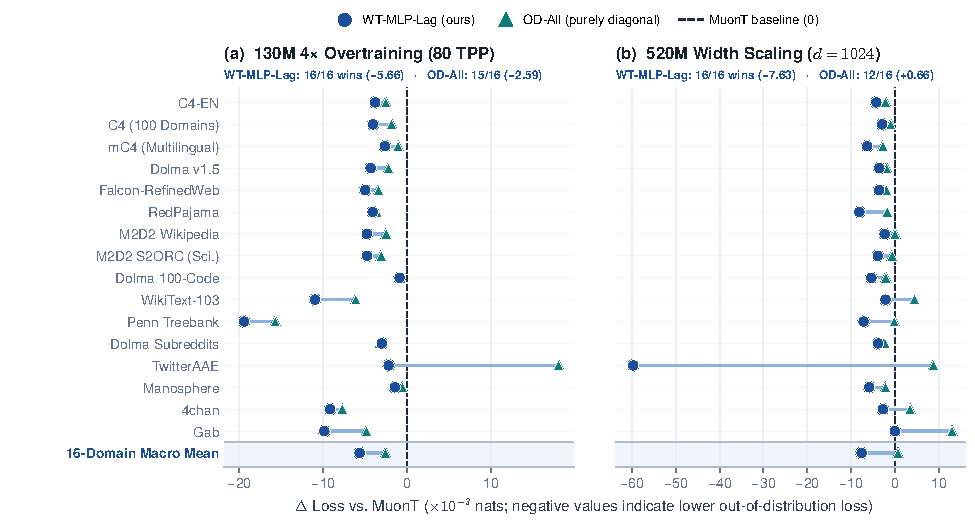
\includegraphics[width=\textwidth]{fig6_paloma_domains.pdf}
 \caption{\textbf{Retaining dense hidden-width output factors improves out-of-distribution loss across Paloma domains.}
 Final per-domain loss differences from \mname{MuonT} (negative values favor the method). \textbf{(a)} At 130M, 80 TPP, \mname{WT-MLP-Lag} wins 16/16 domains. \textbf{(b)} At 520M, 20 TPP, \mname{WT-MLP-Lag} wins 16/16 domains ($-7.63$ mnats macro) while \mname{OD-All} wins 12/16 ($+0.66$ mnats macro). Bottom rows show unweighted 16-domain macro means; horizontal scales differ across panels, and each regime uses one seed.}
 \label{fig:paloma}
\end{figure}

\FloatBarrier
\section{Controls, ablations, and two-sided baselines}
\label{sec:controls_ablations}

Because \mname{MuonT} already removes forward input ill-conditioning, the incremental output-side improvement is a few millinats—a scale where numerical execution differences, short-horizon hyperparameter tuning, or altered regularization can confound optimizer comparisons. We pair execution-path and learning-rate controls with targeted factor-placement ablations and long-horizon comparisons against recent two-sided polar optimizers.

\subsection{Execution-path and learning-rate controls}
\label{sec:falsification}

\mname{Null-WT} executes synchronous cotangent capture, cross-rank pooling, and inverse-root construction identically to the two-sided pipeline, then substitutes identity output factors ($L=\hat L=I$) at the update. While it does not separately test asynchronous scheduling, it directly tests whether altered kernel batching and mixed-precision accumulation manufacture an apparent gain. At $\eta=0.02263$ on 130M seed 0, \mname{Null-WT} finishes just $0.0003$ nats below \mname{MuonT}, compared with $0.0043$ nats for \mname{WT-MLP-Lag} (\Cref{fig:confounds}(b,c), \Cref{tab:controls}), making execution-path drift an unlikely explanation for the improvement.

\begin{figure}[t]
 \centering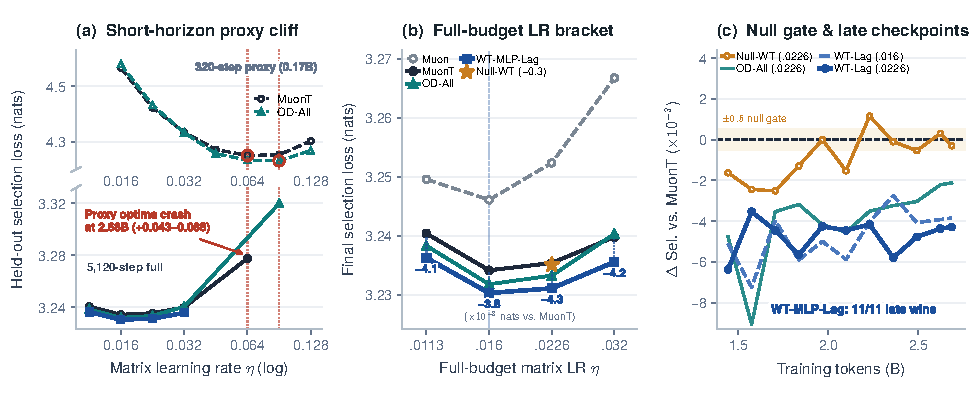
\includegraphics[width=\textwidth]{fig4_confounds_lr_null.pdf}
 \caption{\textbf{The output-side gain survives full-budget learning-rate bracketing and a matched execution-path control.}
 \textbf{(a)} Matrix learning rates chosen on a compressed 320-step proxy sweep transfer poorly to the full 5,120-step budget.
 \textbf{(b)} Full-budget held-out loss across $\eta\in\{0.0113,0.0160,0.0226,0.0320\}$, alongside the matched-path identity control (\mname{Null-WT}).
 \textbf{(c)} Second-half trajectory differences from \mname{MuonT} at $\eta=0.02263$: \mname{Null-WT} stays near zero while \mname{WT-MLP-Lag} wins all 11 late checkpoints. All panels use 130M, seed 0 (2.68B tokens).}
 \label{fig:confounds}
\end{figure}

\begin{table}[tbp]\centering\small
\setlength{\tabcolsep}{5.2pt}
\caption{\textbf{Seed-0 learning-rate bracket, execution-path control, and short-schedule transfer at 130M (2.68B tokens).} Entries are final held-out losses in nats across the complete four-point bracket (bold marks each row's full-budget minimum, $\eta^*=0.0160$ for every method); $\Delta_{0.0226}$ is the paired difference from Muon at $\eta=0.02263$ in millinats where Null-Ctrl is evaluated. The rightmost column transfers each checked arm's 320-step argmax learning rate (\Cref{tab:lr_cliff}) to the full 5,120-step schedule.}\label{tab:controls}
\begin{tabularx}{\textwidth}{@{}>{\raggedright\arraybackslash}Xrrrrrr@{}}
\toprule
& \multicolumn{4}{c}{Full-budget held-out loss $\Lsel$ (nats)} & & \\
\cmidrule(lr){2-5}
Method & $0.0113$ & $0.0160$ & $0.0226$ & $0.0320$ & $\Delta_{0.0226}$ (mnats) & 320-step $\eta^* \to$ full \\
\midrule
Muon & 3.2496 & \textbf{3.2461} & 3.2524 & 3.2667 & $+0.00$ & --- \\
MuonT & 3.2404 & \textbf{3.2342} & 3.2354 & 3.2398 & $-16.96$ & $0.0640 \to 3.2775$ \\
Null-Ctrl & --- & --- & 3.2351 & --- & $-17.26$ & --- \\
Muon2-Diag & 3.2383 & \textbf{3.2318} & 3.2333 & 3.2403 & $-19.08$ & $0.0905 \to 3.3200$ \\
\rowcolor{rowtint}[0pt][0pt]\textbf{Muon2-ExpDiag} & 3.2363 & \textbf{3.2303} & 3.2311 & 3.2356 & $\mathbf{-21.25}$ & --- \\
\bottomrule\end{tabularx}
\end{table}


Short-schedule learning-rate screening is a second major pitfall~\citep{choi2019empirical,schmidt2021crowded,kaddour2023nodata,dang2026batchsize}. A 320-step proxy sweep selects $\eta\in[0.064,0.0905]$—roughly four times the full-budget optimum—and transferring those rates to 5,120 steps degrades final loss by $0.04\text{--}0.09$ nats, swamping second-side differences (\Cref{fig:confounds}(a), \Cref{tab:controls}; complete sweep in \Cref{app:appendix_lr,tab:lr_cliff}). Across the full 2.68B-token bracket $\eta\in\{0.01131,0.016,0.02263,0.032\}$, all four core methods share a strict interior minimum at $\eta^*=0.0160$, and \mname{WT-MLP-Lag} outperforms \mname{MuonT} by $0.0038\text{--}0.0043$ nats at every matched rate.

\subsection{Factor placement, exponent split, and one-step lag}
\label{sec:ablations}

\Cref{tab:ablations} and \Cref{fig:ablations_related}(a) isolate each design element of \mname{WT-MLP-Lag} at 130M (complete 19-arm multi-wave ledger in \Cref{app:ablations,tab:ablations_full}):
\begin{itemize}
 \item \textbf{Dense input whitening remains indispensable.} Replacing input factors with dense output factors alone (\mname{Abl-OutOnly}, $+8.71$ mnats; which also switches weight decay to $\hat L^2 W$) or diagonalizing both sides (\mname{Abl-BothDiag}, $+18.01$ mnats) performs substantially worse than \mname{MuonT}. Diagonalizing the $\dff$-wide \texttt{down} input alongside expanded outputs (\mname{WT-Sym-Lag}, $-1.13$ mnats) likewise sacrifices most of \mname{WT-MLP-Lag}'s gain ($-5.68$ mnats), confirming the input--output asymmetry identified in \Cref{sec:dichotomy}.
 \item \textbf{Both output width classes and both $(-1/2,-1/8)$ factors contribute.} Dropping preconditioning on \texttt{gate,up} (\mname{Abl-No2048}, $-3.07$ mnats) loses roughly half of synchronous \mname{WT-MLP}'s gain ($-6.58$ mnats), whereas upgrading \texttt{gate,up} from diagonal to dense spectral factors (\mname{DT-All}, $-5.78$ mnats) yields no held-out benefit despite raising median step-time overhead to $+21.6\%$. Applying only the post-polar outer factor (\mname{Abl-OuterDense}, $-3.98$ mnats) also underperforms the inner/outer pair.
 \item \textbf{One-step lag retains quality while halving exposed overhead.} Comparing synchronous \mname{WT-MLP} ($-6.58$ mnats) with lagged \mname{WT-MLP-Lag} ($-5.68$ mnats), and synchronous \mname{DT-All} ($-5.78$ mnats) with \mname{DT-All-Lag} ($-5.89$ mnats), retains nearly all of the held-out improvement while cutting unified 8-GPU median step time from $1.221$ to $1.155$\,s ($+11.3\%$ to $+5.3\%$). Because these exploratory arms span implementation waves, they provide provisional component evidence that the fresh-seed campaign in \Cref{sec:scaling} confirms end-to-end.
\end{itemize}

\begin{table}[!htb]\centering\small
\setlength{\tabcolsep}{4.4pt}
\caption{\textbf{Factor-placement, exponent, and scheduling ablations at 130M (seed 0, 2.68B tokens).} Inputs and outputs list the $(\dm / \dff)$ operator assignment under the $(-1/2,-1/8)$ split unless noted; Muon uses $\eta^*=0.016$ and all other arms use $\eta=0.02263$. Loss columns report cohort-adjusted 11-checkpoint second-half mean differences (millinats) relative to Muon (negative favors the row method; MuonT sits at $-5.50$ and $-5.34$ mnats). Step $\Delta t$ is median step-time overhead relative to Muon in the unified 8-GPU benchmark (\Cref{tab:bench19}), matching \Cref{fig:mech_pareto}(b,c). All 19 exploratory arms appear in \Cref{tab:ablations_full}.}\label{tab:ablations}
\begin{tabularx}{\textwidth}{@{}>{\raggedright\arraybackslash}Xllcrrr@{}}
\toprule
Method & Inputs ($\dm / \dff$) & Outputs ($\dm / \dff$) & Lag & Late $\Delta\Lsel$ & Late $\Delta\Lc$ & Step $\Delta t$ \\
\midrule
\addlinespace[2pt]\multicolumn{7}{@{}l}{\textit{Reference baselines and execution-path control}}\\
Muon & $I$ / $I$ & $I$ / $I$ & --- & $+0.00$ & $+0.00$ & $+0.0\%$ \\
MuonT & Dense / Dense & $I$ / $I$ & --- & $-5.50$ & $-5.34$ & $+1.5\%$ \\
Null-Ctrl & Dense / Dense & $I$ / $I$ (solved) & 0 & $-6.15$ & $-7.39$ & $+13.9\%$ \\
\addlinespace[4pt]\multicolumn{7}{@{}l}{\textit{Replacing or weakening input whitening}}\\
Abl-BothDiag & Diag / Diag & Diag / Diag & 0 & $+12.51$ & $+12.34$ & $+1.1\%$ \\
Abl-OutOnly & $I$ / $I$ & Dense / Dense & 0 & $+3.20$ & $+5.55$ & $+31.7\%$ \\
Abl-SymDiag & Dense / Diag & Dense / Diag & 1 & $-6.63$ & $-6.95$ & $+4.8\%$ \\
\addlinespace[4pt]\multicolumn{7}{@{}l}{\textit{Output projection role and inner/outer exponent placement}}\\
Abl-NoExp & Dense / Dense & Dense / $I$ & 0 & $-8.57$ & $-7.97$ & $+13.7\%$ \\
Abl-OuterDense & Dense / Dense & $\hat L$ Dense ($L=I$) & 0 & $-9.48$ & $-10.12$ & $+28.2\%$ \\
Muon2-Diag & Dense / Dense & Diag / Diag & 0 & $-10.01$ & $-8.95$ & $+3.7\%$ \\
\addlinespace[4pt]\multicolumn{7}{@{}l}{\textit{Dense two-sided ceiling versus expansion-diagonal outputs and one-step lag}}\\
Muon2-Dense & Dense / Dense & Dense / Dense & 0 & $-11.29$ & $-11.72$ & $+23.3\%$ \\
Muon2-Dense (lag) & Dense / Dense & Dense / Dense & 1 & $-11.40$ & $-11.21$ & $+18.2\%$ \\
Muon2-ExpDiag (sync) & Dense / Dense & Dense / Diag & 0 & $\mathbf{-12.09}$ & $-11.42$ & $+12.9\%$ \\
\rowcolor{rowtint}[0pt][0pt]\textbf{Muon2-ExpDiag} & Dense / Dense & Dense / Diag & 1 & $\mathbf{-11.19}$ & $\mathbf{-10.33}$ & $+6.8\%$ \\
\bottomrule\end{tabularx}
\end{table}


\begin{figure}[t]
 \centering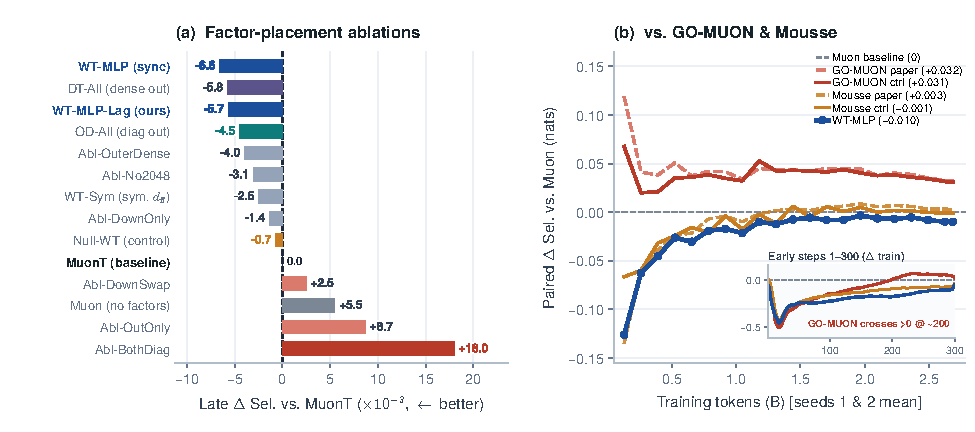
\includegraphics[width=\textwidth]{fig7_ablations_and_related.pdf}
 \caption{\textbf{Width-thresholded output preconditioning outperforms factor-placement ablations and alternative two-sided polar baselines.}
 \textbf{(a)} Second-half held-out loss differences from cohort \mname{MuonT} across 14 configurations at 130M, 2.68B tokens (seed 0; exploratory multi-wave settings in \Cref{tab:ablations,tab:ablations_full}).
 \textbf{(b)} Held-out trajectories relative to \mname{Muon} under shared isotropic matrix decay ($\lambda=0.1,\eta=0.032$, mean of fresh seeds 1 and 2). Inset: early training loss over steps 1--300, where \mname{GO-MUON}'s initial lead reverses near step 200 while \mname{WT-MLP} retains its advantage through 2.68B tokens.}
 \label{fig:ablations_related}
\end{figure}

\subsection{Comparison with two-sided polar baselines}
\label{sec:related_baselines}

We also compare synchronous \mname{WT-MLP} against two recent methods that combine second-order statistics with polar updates: \mname{GO-MUON}~\citep{che2026gomuon}, which applies symmetric $(-1/4,-1/4)$ activation/cotangent powers with norm grafting, and \mname{Mousse}~\citep{zhang2026mousse}, which applies symmetric $(-1/8,-1/8)$ powers of full gradient Gram matrices $GG^{\Tr}$ and $G^{\Tr}G$ with norm grafting. For each baseline, we evaluate both a controlled profile sharing our EMA, damping, refresh cadence, and $\Nten$ map, and a paper profile following method-specific choices, under shared isotropic matrix decay ($\lambda=0.1,\eta=0.032$) across two fresh seeds (\Cref{tab:related}, \Cref{fig:ablations_related}(b); a controlled recipe comparison rather than independent hyperparameter tuning).

\begin{table}[!htb]\centering\small
\setlength{\tabcolsep}{4.2pt}
\caption{\textbf{Two-sided polar baselines under a shared isotropic-decay recipe (130M, 2.68B tokens).} Entries average fresh seeds 1 and 2 at $\eta=0.032$ and $\lambda=0.1$ on the standalone synchronous harness. Held-out is final $\Lsel$ in nats; $\Delta$ columns are millinats from Muon (Late-11 averages the second-half checkpoints); Step is median seconds per update.}\label{tab:related}
\begin{tabularx}{\textwidth}{@{}ll>{\raggedright\arraybackslash}Xrrrrr@{}}
\toprule
Method & Profile & Moments \& Exponents & Held-out & $\Delta\Lsel$ & Late-11 $\Delta$ & $\Delta\Lc$ & Step (s) \\
\midrule
Muon & Reference & None; $\Nten(U)$ & 3.2074 & $+0.00$ & $+0.00$ & $+0.00$ & 1.15 \\
Mousse & Paper & $GG^{\Tr}, G^{\Tr}G$; $(-1/8,-1/8)$ + graft & 3.2102 & $+2.78$ & $+4.85$ & $+3.25$ & 1.13 \\
Mousse & Controlled & $GG^{\Tr}, G^{\Tr}G$; $(-1/8,-1/8)$ + graft & 3.2064 & $-0.98$ & $+1.23$ & $-1.92$ & 1.20 \\
GO-MUON & Controlled & $C, B$; $(-1/4,-1/4)$ + graft & 3.2384 & $+30.98$ & $+38.22$ & $+29.36$ & 1.59 \\
GO-MUON & Paper & OAS $C, B$; SVD + graft & 3.2395 & $+32.08$ & $+39.71$ & $+30.48$ & 2.02 \\
\rowcolor{rowtint}[0pt][0pt]\textbf{Muon2-ExpDiag} & Sync ($\tau=0$) & $C, B$ (\texttt{gate,up} diag); $(-1/2,-1/8)$ & \textbf{3.1975} & $\mathbf{-9.90}$ & $\mathbf{-7.14}$ & $\mathbf{-9.91}$ & 1.36 \\
\bottomrule\end{tabularx}
\end{table}


At 2.68B tokens, both \mname{GO-MUON} profiles finish roughly $0.03$ nats worse than \mname{Muon}—reversing an early 200-step training-loss lead—while both \mname{Mousse} profiles finish close to \mname{Muon}. Under the same isotropic decay, \mname{WT-MLP} lowers held-out loss by $0.0099$ nats below \mname{Muon}, showing that its benefit does not depend on \mname{MuonT}'s shaped weight decay. Two operator differences are consistent with this gap: a gradient Gram $GG^{\Tr}=\sum_{i,j}\langle x_i,x_j\rangle\delta_i\delta_j^{\Tr}$ entangles cotangents with activation inner products and cross-token terms that separate $(C,B)$ moments avoid, and steeper $(-1/4,-1/4)$ outer inverse powers with norm grafting place heavier weight on noisy low-variance cotangent modes—though because these baselines change multiple choices together, this comparison does not isolate a single causal factor.

\FloatBarrier
\section{Optimization mechanism and systems cost}
\label{sec:mechanism_cost}

\paragraph{From loss gains to update geometry and runtime.}
We next examine how structure-aware output factors change individual parameter updates and multi-checkpoint cotangent trajectories, and measure the remaining step-time overhead across GPU counts.

\subsection{Output factors rotate updates with little norm change}
\label{sec:mechanism}

\paragraph{Counterfactual step-norm invariance.}
To isolate the immediate action of the output operator, we hold checkpoint momentum and input factors fixed and recompute counterfactual updates under identity (\mname{MuonT}), all-diagonal (\mname{Muon2-Diag}), and expansion-diagonal (\mname{Muon2-ExpDiag}) output factors on saved 130M (32 layers, step 2,500) and 520M ($\eta^*=0.016$, 16 layers, step 5,120) checkpoints (\Cref{tab:mechanism_rotation}, \Cref{fig:mech_pareto}(a)). Across projections, \mname{Muon2-ExpDiag} update Frobenius norms stay at $0.985\times$ their input-only counterparts at 130M and $1.006\times$ at 520M, ruling out global step-size inflation.

\paragraph{Stiefel frame rotation from inner whitening.}
An exact row-polar identity shows why inner whitening rotates the update even after singular values are equalized. For a full-row-rank pre-polar matrix $Z_0=UR=S_0P_0$ with $m\le n$, $S_0\succ0$, and $P_0P_0^{\Tr}=I_m$, left-multiplying by $L\succ0$ gives
\begin{equation}
 \operatorname{Polar}(LZ_0)=\Omega P_0,\qquad
 \Omega=(LS_0^2L)^{-1/2}LS_0\in SO(m).
 \label{eq:som_rotation}
\end{equation}
Whenever $L$ and $S_0$ do not commute, $\Omega$ rotates the orthogonal row frame tangentially along the Stiefel manifold, while post-multiplying by symmetric $\hat L$ scales output directions orthogonally in first-order Frobenius inner product ($\tr(HK^{\Tr})=0$ for symmetric $H$ and skew-symmetric $K$; derivations and empirical inner/outer angles for finite $\Nten$ and tall matrices appear in \Cref{app:appendix_mech,tab:rotation_detail}).

\begin{table}[!htb]\centering\small
\setlength{\tabcolsep}{4.5pt}
\caption{\textbf{Counterfactual update rotation, top-mode de-hijacking, and width scaling across 130M (32-layer means) and 520M (16-layer means).} Holding checkpoint momentum and input factors fixed, $\theta_{\rm WT}$ and $\theta_{\rm OD}$ measure update angles relative to input-only updates ($\|D_{\rm WT}\|_F/\|D_{\rm MT}\|_F = 0.985$ at 130M and $1.006$ at 520M). Hijack reports top-16 overlap between pre-polar momentum singular vectors and $B_t$ eigenvectors before and after inner whitening; DA is 520M median diagonal anisotropy share (residual $\mathrm{IPR}=3.02$); $\Phi$ ratios are directional quadratic proxies relative to MuonT, not measured loss gains. At 520M, \texttt{gate,up} track 1D diagonals online ($\text{WT}=\text{OD}$).}\label{tab:mechanism_rotation}
\begin{tabularx}{\textwidth}{@{}>{\raggedright\arraybackslash}Xrrrrrrrrr@{}}
\toprule
& \multicolumn{4}{c}{130M ($\dm=512$, step 2,500)} & \multicolumn{5}{c}{520M ($\dm=1{,}024$, step 5,120)} \\
\cmidrule(lr){2-5}\cmidrule(lr){6-10}
Output & Hijack & $\theta_{\rm WT}$ & $\theta_{\rm OD}$ & $\Phi_{\rm WT}/\Phi_{\rm MT}$ & DA & $\theta_{\rm WT}$ & $\theta_{\rm OD}$ & $\Phi_{\rm WT}/\Phi_{\rm MT}$ & $\Phi_{\rm OD}/\Phi_{\rm MT}$ \\
\midrule
q & $67.8\to2.8\%$ & $22.7^\circ$ & $20.8^\circ$ & 1.155 & 9.8\% & $24.0^\circ$ & $22.7^\circ$ & 1.625 & 1.182 \\
k & $64.2\to3.7\%$ & $22.6^\circ$ & $22.8^\circ$ & 1.233 & 16.8\% & $24.8^\circ$ & $24.5^\circ$ & 1.737 & 1.247 \\
v & $19.6\to1.1\%$ & $24.2^\circ$ & $17.2^\circ$ & 1.264 & 0.7\% & $25.1^\circ$ & $16.5^\circ$ & 3.341 & 1.137 \\
\addlinespace[2.5pt]
\rowcolor{rowtint}[0pt][0pt]\textbf{o} (res.) & $30.4\to3.5\%$ & $15.5^\circ$ & $3.9^\circ$ & 1.002 & 0.5\% & $\mathbf{15.4^\circ}$ & $6.4^\circ$ & \textbf{1.334} & 1.028 \\
\rowcolor{rowtint}[0pt][0pt]\textbf{down} (res.) & $64.5\to2.8\%$ & $15.7^\circ$ & $5.1^\circ$ & 1.098 & 0.4\% & $\mathbf{14.6^\circ}$ & $6.0^\circ$ & \textbf{1.263} & 1.009 \\
\addlinespace[2.5pt]
gate & $22.7\to3.1\%$ & $15.9^\circ$ & $15.9^\circ$ & 1.292 & --- & $18.8^\circ$ & $18.8^\circ$ & --- & --- \\
up & $33.7\to4.7\%$ & $16.4^\circ$ & $16.4^\circ$ & 1.249 & --- & $18.6^\circ$ & $18.6^\circ$ & --- & --- \\
\bottomrule\end{tabularx}
\end{table}


\begin{figure}[t]
 \centering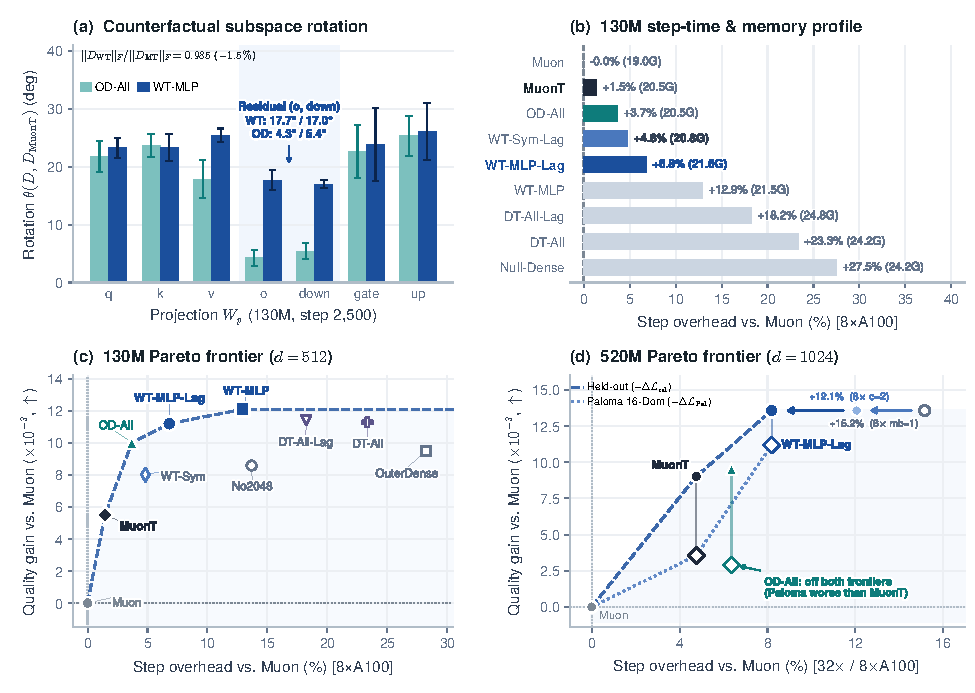
\includegraphics[width=\textwidth]{fig8_mechanism_and_pareto.pdf}
 \caption{\textbf{Dense output factors rotate residual-stream updates while retaining a bounded runtime cost.}
 \textbf{(a)} Counterfactual update rotation relative to input-only updates at 130M, step 2,500 (each arm on its own trained state; bars show 32-layer means and whiskers $\pm1$ SD; common-state probes at both widths are in \Cref{tab:mechanism_rotation}).
 \textbf{(b)} 130M median step-time overhead versus \mname{Muon} and per-GPU peak memory on $8\times\text{A100}$.
 \textbf{(c, d)} Quality gain versus median step-time overhead at 130M ($8\times\text{A100}$) and 520M ($32\times$ and $8\times\text{A100}$). Frontiers combine fixed-token losses with steady-step timing benchmarks rather than wall-clock time to a target loss.}
 \label{fig:mech_pareto}
\end{figure}

\paragraph{Residual update rotation and singular-frame de-hijacking.}
On the 520M checkpoint, \mname{Muon2-ExpDiag} rotates the residual-stream \texttt{o} and \texttt{down} updates by $15.4^\circ$ and $14.6^\circ$, compared with $6.4^\circ$ and $6.0^\circ$ under \mname{Muon2-Diag} (\Cref{tab:mechanism_rotation}). At 130M, inner whitening cuts top-16 overlap between pre-polar momentum singular vectors and dominant $B_t$ eigenvectors from $30\text{--}68\%$ to $2.8\text{--}3.7\%$ ($19.6\to1.1\%$ on \texttt{v}) while raising row alignment across 69--82\% of the trailing 80\% of output modes (\Cref{tab:rotation_detail}). Structure-aware updates also raise the directional quadratic score $\Phi_{B,C}(\hat D)=\langle U,\hat D\rangle^2/\tr(\tilde B\hat D\tilde C\hat D^{\Tr})$ over \mname{MuonT}. Because observed-label cotangent moments are not true Hessians or model Fishers~\citep{kunstner2019limitations} (and \mname{GO-MUON} can score high on $\Phi_{B,C}$ despite poor training loss), these probes describe update geometry rather than proving causal generalization gains.

\paragraph{Eigenvector delocalization across model width.}
Coordinate scaling misses more of these residual rotations as width grows because residual-output eigenvectors are spread across coordinates. Their median normalized inverse participation ratio is $d\sum_i u_i^4\approx 3.01\text{--}3.02$ at both widths, close to the Haar-random benchmark $3d/(d+2)$. Under a reference model with Haar-distributed eigenvectors and fixed non-isotropic eigenvalues, expected diagonal anisotropy decays inversely with width:
\begin{equation}
 \E_{U\sim\mathrm{Haar}}[\mathrm{DiagAniso}(U\Lambda U^{\Tr})]=\frac{2}{d+2},
 \label{eq:haar_scaling}
\end{equation}
matching the observed drop in residual-output diagonal share from $\approx 0.8\%$ at $\dm=512$ to $0.45\%$ at $\dm=1{,}024$.

\subsection{Trajectory-level reduction in output-subspace drift}
\label{sec:output_drift}

\paragraph{Fixed-data subspace-drift protocol.}
Training with \mname{Muon2-ExpDiag} also slows the temporal drift of leading output-cotangent subspaces across saved checkpoints (\Cref{tab:output_drift}, \Cref{fig:output_drift}). To compare all seven output roles on shared data without minibatch-order noise, we evaluate each saved checkpoint passively on two disjoint fixed sets $\mathcal S$ of 4,576 token positions (16 windows of 4,096 tokens each) to form $B_t^{\mathcal S}=|\mathcal S|^{-1}\sum_{s\in\mathcal S}\delta_t(s)\delta_t(s)^{\Tr}$ for each projection. Between consecutive checkpoints, we measure principal-angle subspace drift $D_k(t_1,t_2)=1-\|V_{t_1}^{\Tr}V_{t_2}\|_F^2/k$ at $k=16$ (full protocol, per-role curves, EMA audit, and sensitivity checks in \Cref{app:drift_details,fig:output_drift_roles}).

\begin{table}[tbp]\centering\footnotesize
\setlength{\tabcolsep}{5pt}
\caption{\textbf{Output-subspace drift with Muon as the baseline.} Fixed-data top-16 drift, averaged equally over 32 layers, two probe sets, and 19 intervals of 250 steps at 130M or three intervals of 2,560 steps at 520M. At 520M and in fresh 130M seeds 1--3 (one 2,560--5,120 interval per seed), all three methods share $\eta=0.016$; the densely saved 130M seed-0 trajectories use $0.016$ for Muon and $0.02263$ for MuonT/WT, so that column does not isolate optimizer effects at a common rate. Reductions are $100(1-\overline D_{\rm method}/\overline D_{\rm Muon})$; positive values mean lower drift than Muon. Seed summaries are mean $\pm$ sample SD across three seeds. The all-role row averages drift before taking ratios; absolute drift is not compared across model sizes. WT denotes WT-MLP-Lag.}\label{tab:output_drift}
\begin{tabularx}{\textwidth}{@{}>{\raggedright\arraybackslash}X*{6}{>{\raggedleft\arraybackslash}X}@{}}\toprule
& \multicolumn{3}{c}{130M: absolute drift} & \multicolumn{3}{c}{520M: absolute drift} \\
\cmidrule(lr){2-4}\cmidrule(lr){5-7}
Output & Muon & MuonT & WT & Muon & MuonT & WT \\\midrule
\texttt{q} & 0.363 & 0.368 & 0.304 & 0.352 & 0.348 & 0.277 \\
\texttt{k} & 0.399 & 0.390 & 0.366 & 0.494 & 0.469 & 0.431 \\
\texttt{v} & 0.565 & 0.614 & 0.591 & 0.771 & 0.762 & 0.745 \\
\texttt{o} & 0.335 & 0.360 & 0.284 & 0.529 & 0.461 & 0.410 \\
\texttt{down} & 0.313 & 0.342 & 0.276 & 0.493 & 0.426 & 0.393 \\
\texttt{gate} & 0.682 & 0.677 & 0.522 & 0.863 & 0.837 & 0.665 \\
\texttt{up} & 0.583 & 0.583 & 0.358 & 0.764 & 0.746 & 0.471 \\
\midrule
All roles & 0.463 & 0.476 & 0.386 & 0.609 & 0.579 & 0.485 \\
\bottomrule\end{tabularx}
\par\vspace{6pt}
\begin{tabularx}{\textwidth}{@{}>{\raggedright\arraybackslash}Xrrrrrr@{}}\toprule
& \multicolumn{2}{c}{130M: reduction (\%)} & \multicolumn{2}{c}{520M: reduction (\%)} & \multicolumn{2}{c}{130M seeds 1--3: reduction (\%)} \\
\cmidrule(lr){2-3}\cmidrule(lr){4-5}\cmidrule(lr){6-7}
Output & MuonT & WT & MuonT & WT & MuonT & WT \\\midrule
\texttt{q} & -1.6 & +16.2 & +1.1 & +21.3 & $+2.7\pm1.1$ & $+17.5\pm2.7$ \\
\texttt{k} & +2.3 & +8.4 & +5.1 & +12.7 & $+5.9\pm1.5$ & $+8.9\pm0.8$ \\
\texttt{v} & -8.7 & -4.6 & +1.1 & +3.3 & $+2.0\pm0.6$ & $+3.2\pm0.8$ \\
\texttt{o} & -7.4 & +15.2 & +12.8 & +22.6 & $+2.2\pm6.3$ & $+19.2\pm2.1$ \\
\texttt{down} & -9.0 & +12.1 & +13.6 & +20.4 & $+1.4\pm7.9$ & $+16.4\pm1.9$ \\
\texttt{gate} & +0.7 & +23.6 & +3.0 & +22.9 & $+5.3\pm2.3$ & $+22.6\pm1.1$ \\
\texttt{up} & 0.0 & +38.6 & +2.3 & +38.4 & $+2.7\pm3.2$ & $+39.5\pm0.8$ \\
\midrule
All roles & -2.9 & +16.7 & +5.1 & +20.5 & $+3.3\pm2.9$ & $+18.8\pm0.6$ \\
\bottomrule\end{tabularx}
\end{table}


\begin{figure}[tbp]
 \centering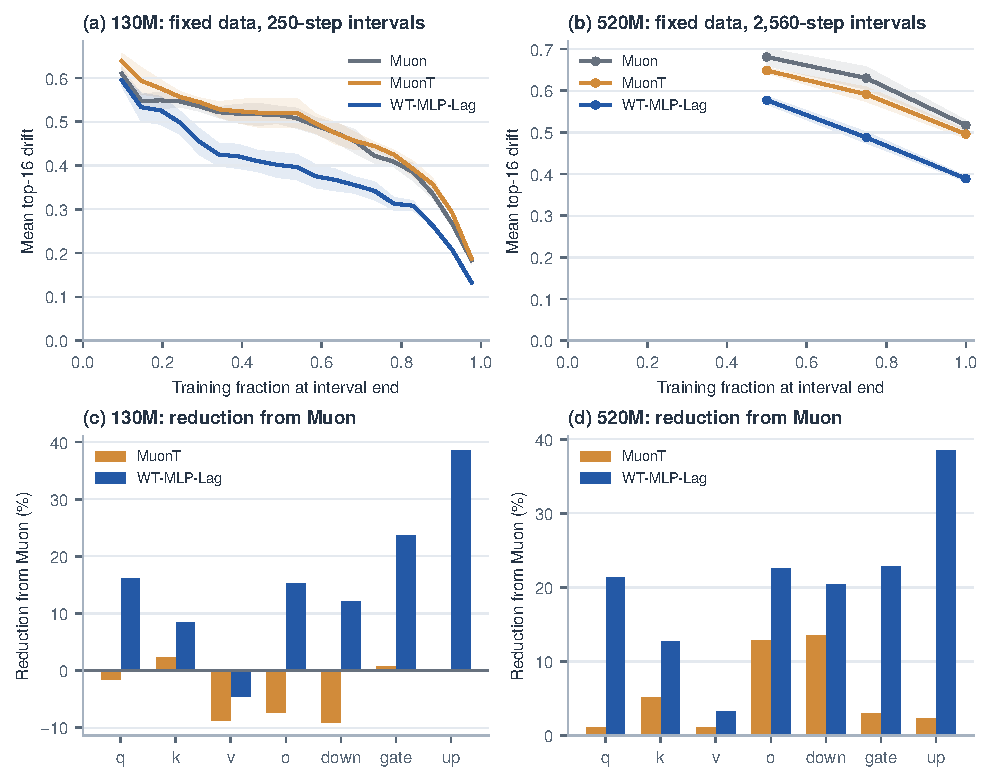
\includegraphics[width=\textwidth]{fig9_output_drift.pdf}
 \caption{\textbf{\mname{Muon2-ExpDiag} reduces leading output-subspace drift across 130M and 520M training trajectories.}
 \textbf{(a, b)} Fixed-data top-16 cotangent-subspace drift across saved \mname{Muon}, \mname{MuonT}, and \mname{Muon2-ExpDiag} checkpoints, averaged over seven output roles, 32 layers, and two disjoint probe sets (shading spans the two probe-set means; 19 intervals of 250 steps at 130M and three 2,560-step intervals at 520M).
 \textbf{(c, d)} Role-wise percentage drift reduction relative to \mname{Muon}. All three 520M runs share $\eta=0.016$, whereas 130M seed-0 runs use $\eta=0.016$ for \mname{Muon} and $\eta=0.02263$ for \mname{MuonT} and \mname{Muon2-ExpDiag}; matched-rate fresh-seed checks appear in \Cref{tab:output_drift}.}
 \label{fig:output_drift}
\end{figure}

\paragraph{Drift reductions across 130M and 520M trajectories.}
Relative to \mname{Muon}, \mname{Muon2-ExpDiag} lowers all-role mean top-16 drift by 16.7\% across 19 equal 250-step intervals at 130M ($0.463\to0.386$, whereas \mname{MuonT} is $2.9\%$ higher at $0.476$), and by 20.5\% across the three 2,560-step intervals covering the final three quarters of matched-rate ($\eta=0.016$) 520M training ($0.609\to0.485$, versus $0.579$ or $+5.1\%$ reduction for \mname{MuonT}). Reductions are largest on \texttt{gate} ($23.6\%,22.9\%$) and \texttt{up} ($38.6\%,38.4\%$); at 520M every role decreases in every interval (including $+3.3\%$ on \texttt{v}), whereas on the mixed-rate 130M seed-0 curve \texttt{v} sits $-4.6\%$ higher than \mname{Muon}. Relative to \mname{MuonT}, \mname{Muon2-ExpDiag} lowers all-role drift by 19.0\% at 130M and 16.2\% at 520M, improving every role in every equal-length interval. Because the densely saved 130M seed-0 runs use $\eta=0.016$ for \mname{Muon} and $\eta=0.02263$ for \mname{MuonT} and \mname{Muon2-ExpDiag}, we also check the three fresh 130M seeds at matched $\eta=0.016$ (steps 2,560--5,120): as at 520M, \mname{Muon2-ExpDiag} reduces drift relative to \mname{Muon} across all seven roles on every seed, averaging $18.8\pm0.6\%$ overall versus $3.3\pm2.9\%$ for \mname{MuonT}.

\paragraph{Training-EMA and rank-sensitivity checks.}
Uninterrupted 130M training-EMA checkpoints relative to a passive \mname{MuonT} control confirm lower average top-16 drift across all five saved dense output roles ($16.3\%,12.0\%,11.4\%,7.8\%,28.0\%$ on \texttt{q,k,v,o,down}), while qualifying \Cref{tab:diagnosis_summary}'s resumed replay window where uninterrupted steps 2,250--2,500 are slightly higher on \texttt{o,down} ($0.138,0.109$ versus $0.134,0.107$) despite lower full-run averages. Fixed-data sign patterns also hold across $k\in\{8,16,32,64\}$ and under a 1\% eigenvalue-gap filter (\Cref{app:drift_details}). These audits measure trajectory subspace stability; they do not establish that lower drift causes lower held-out loss or permits slower root refreshes.

\subsection{Step-time overhead and token-versus-time tradeoff}
\label{sec:pareto}

\paragraph{Median step-time waterfall across GPU scales.}
Expansion-output diagonalization and one-step overlap remove most, though not all, of two-sided runtime cost (\Cref{tab:timing_summary}, \Cref{fig:mech_pareto}(b--d); excluding compilation, evaluation, and checkpoint I/O). On matched 130M checkpoints ($8\times\text{A100}$), input-only \mname{MuonT} adds $+1.5\%$ median step time over \mname{Muon} and synchronous dense outputs (\mname{Muon2-Dense}) add $+23.3\%$; diagonalizing \texttt{gate,up} (\mname{Muon2-ExpDiag (sync)}) cuts total overhead to $+12.9\%$, and one-step lag (\mname{Muon2-ExpDiag}) lowers it to $+6.8\%$ ($+5.3\%$ above \mname{MuonT}). At 520M across $32\times\text{A100}$, matched-checkpoint median overhead over \mname{Muon} is $+4.8\%$ for \mname{MuonT} and $+8.2\%$ for \mname{Muon2-ExpDiag} ($+3.3\%$ above \mname{MuonT}).

\begin{table}[!htb]\centering\small
\setlength{\tabcolsep}{5.8pt}
\caption{\textbf{Step-time co-design waterfall and multi-node scaling (both median and mean estimators).} Overheads ($\Delta$) are relative to same-group Muon using the matching estimator (matching \Cref{fig:overview}(b) and \Cref{fig:mech_pareto}(b--d)); Peak GiB is per-GPU peak allocated memory. Expansion-output diagonalization and one-step lag cut total two-sided median overhead from $+23.3\%$ (Muon2-Dense) to $+6.8\%$ at 130M ($+5.3\%$ above MuonT) and $+8.2\%$ at 520M ($+3.3\%$ above MuonT), while retaining a slower mean tail from periodic basis repairs. Complete 130M and 520M configurations appear in \Cref{tab:bench19,tab:bench520m}.}\label{tab:timing_summary}
\begin{tabularx}{\textwidth}{@{}>{\raggedright\arraybackslash}Xrrrrr@{}}
\toprule
Configuration / Method & Median (s) & Median $\Delta$ & Mean (s) & Mean $\Delta$ & Peak GiB \\
\midrule
\addlinespace[2pt]\multicolumn{6}{@{}l}{\textit{130M co-design progression: 8 GPUs, 0.5M batch, matched checkpoint (steps 37--96)}}\\
Muon (reference) & 1.081 & $+0.0\%$ & 1.079 & $+0.0\%$ & 18.97 \\
MuonT (input only) & 1.097 & $+1.5\%$ & 1.097 & $+1.7\%$ & 20.54 \\
Muon2-Diag (all outputs diagonal) & 1.121 & $+3.7\%$ & 1.120 & $+3.7\%$ & 20.55 \\
Muon2-Dense (all outputs dense, sync) & 1.333 & $+23.3\%$ & 1.459 & $+35.2\%$ & 24.21 \\
Muon2-ExpDiag (sync, $\tau=0$) & 1.221 & $+12.9\%$ & 1.250 & $+15.8\%$ & 21.52 \\
\rowcolor{rowtint}[0pt][0pt]\textbf{Muon2-ExpDiag ($\tau=1$ lag)} & \textbf{1.155} & $\mathbf{+6.8\%}$ & \textbf{1.194} & $\mathbf{+10.7\%}$ & \textbf{21.60} \\
\addlinespace[5pt]\multicolumn{6}{@{}l}{\textit{520M width and cluster scaling: 32 GPUs, 1.0M batch, chunked buffers}}\\
Muon (matched ckpt, ref.) & 1.322 & $+0.0\%$ & 1.324 & $+0.0\%$ & 26.46 \\
MuonT (matched ckpt) & 1.385 & $+4.8\%$ & 1.391 & $+5.1\%$ & 26.93 \\
Muon2-Diag (matched ckpt) & 1.406 & $+6.4\%$ & 1.412 & $+6.6\%$ & 26.94 \\
\rowcolor{rowtint}[0pt][0pt]\textbf{Muon2-ExpDiag (matched ckpt)} & \textbf{1.430} & $\mathbf{+8.2\%}$ & \textbf{1.549} & $\mathbf{+17.0\%}$ & \textbf{27.88} \\
Muon2-ExpDiag (warm vs.\ warm Muon) & 1.458 & $+11.1\%$ & 1.539 & $+16.9\%$ & 27.88 \\
\bottomrule\end{tabularx}
\end{table}


\paragraph{Upper-tail repair cost and wall-clock tradeoff.}
Periodic fallback eigendecompositions leave a heavier upper tail in mean step times: relative to \mname{Muon}, the same matched benchmarks record mean overheads of $+10.7\%$ at 130M and $+17.0\%$ at 520M, or $+8.9\%$ and $+11.4\%$ above \mname{MuonT} ($+11.1\%$ median and $+16.9\%$ mean vs.\ warm \mname{Muon}, or $+5.6\%$ and $+11.1\%$ above warm \mname{MuonT}, when resuming each method's own warmed 520M state on 32 GPUs; complete 8- and 32-GPU windows in \Cref{tab:bench19,tab:bench520m}). At a recorded 130M C4 target of $3.52$ nats, \mname{Muon2-ExpDiag} reaches the target in $5.3\%$ fewer tokens than \mname{MuonT} (step 4,501 vs.\ 4,751; $2.36\text{B}$ vs.\ $2.49\text{B}$ tokens) but $1.8\%$ more elapsed wall-clock time ($5{,}564.6$ vs.\ $5{,}468.4$\,s). Our experiments therefore establish a fixed-token quality improvement while leaving net wall-clock speedups open.

\FloatBarrier
\section{Related work}
\label{sec:related}

\paragraph{Polar momentum and input-side preconditioning.}
\mname{Muon} introduced Newton--Schulz orthogonalization of matrix momentum~\citep{jordan2024muon}, motivating recent analyses of singular-value flattening, update norms, and subspace alignment~\citep{shumaylov2026freon,goyal2026spectrally}. Our counterfactual probes build on this separation between step norm and update direction. On the input side, \mname{Newton-Muon} studies when polar orthogonalization cancels left curvature~\citep{du2026newtonmuon}, \mname{MuonT} (Toner) introduces decoupled $(-1/2,-1/8)$ input activation inverse powers with cached-eigenbasis tracking~\citep{mohamadi2026toner}, and \mname{MuonH} replaces decoupled weight decay with Frobenius sphere retraction~\citep{wen2026hyperball} (\Cref{sec:hyperball}). \mname{Muon2-ExpDiag} extends \mname{MuonT} to make output-side preconditioning fast and measurable.

\paragraph{Kronecker, Gram, and two-sided polar preconditioners.}
Two-sided preconditioning has deep roots outside polar optimizers: \mname{K-FAC} factors curvature into activation and cotangent second moments~\citep{martens2015kfac}, while \mname{Shampoo} and \mname{SOAP} maintain left and right gradient Gram preconditioners~\citep{gupta2018shampoo,anil2020scalable,vyas2024soap}. Concurrent polar methods such as \mname{GO-MUON} and \mname{Mousse} apply symmetric moment or gradient-Gram inverse powers around orthogonalization with norm grafting~\citep{che2026gomuon,zhang2026mousse}. Rather than treating every projection alike, we assign dense or diagonal output factors by projection role, retain right-only weight decay, overlap output roots at a one-step lag, and test against execution-path controls, without claiming that cotangent moments outperform gradient statistics across all architectures or tuning regimes.

\section{Conclusion and scope}
\label{sec:conclusion}

\paragraph{Summary of contributions.}
\mname{Muon2-ExpDiag} shows that output-cotangent preconditioning improves a \mname{Muon} optimizer that already whitens its inputs, provided factor fidelity and scheduling match Transformer block geometry. Dense $(-1/2,-1/8)$ output roots at hidden width supply the cross-channel rotations needed by residual-stream writers, exact diagonal scaling on gated SwiGLU expansion outputs removes 96.2\% of nominal cubic output work where anisotropy is coordinate-aligned, right-only weight decay avoids late-cooldown degradation from output-shaped shrinkage, and a one-step side-stream lag overlaps output reductions and root repairs with training. Across three fresh 130M seeds, fourfold horizon scaling to 10.74B tokens, and width transfer to 520M, \mname{Muon2-ExpDiag} lowers held-out and out-of-distribution losses below tuned \mname{MuonT}, whereas all-diagonal output scaling (\mname{Muon2-Diag}) adds almost no held-out gain and regresses out of distribution at greater width.

\paragraph{Limitations and future directions.}
Several scope limits remain. The 80-TPP and 520M scaling runs each use one seed, all runs study a single pre-RMSNorm SwiGLU architecture family up to 537M non-embedding parameters, and our counterfactual and subspace-drift probes remain descriptive checkpoint audits rather than a causal proof of generalization. Periodic eigenbasis repairs also keep mean step-time overhead above median overhead ($10.7\text{--}17.0\%$ vs.\ $6.8\text{--}11.1\%$ over \mname{Muon}, or $8.9\text{--}11.4\%$ vs.\ $3.3\text{--}5.6\%$ above \mname{MuonT}), so fixed-token loss reductions do not yet yield wall-clock speedups. Head-block output approximations, adaptive root-refresh schedules, and multi-seed evaluations at multi-billion-parameter scale are natural next steps.


\FloatBarrier
\bibliographystyle{plainnat}
\bibliography{refs}

\clearpage
\appendix
\crefalias{section}{appendix}
\section{Numerical operator and implementation}
\label{app:appendix_math}

\subsection{Finite Newton--Schulz map}

The executed map uses ten polynomial iterations in mixed precision, so it is not an exact SVD polar factor. For $Z=LUR$, we first compute $X_0=Z/(\|Z\|_F+10^{-5})$ in FP32. Tall matrices are transposed so each Gram has dimension $\min(m,n)$. For $k=0,\ldots,9$,
\begin{equation}
 A_k=X_k\star X_k^{\Tr},\qquad
 X_{k+1}=3.4445X_k+[-4.7750A_k+2.0315(A_k\star A_k)]\star X_k,
 \label{eq:ns10}
\end{equation}
where $P\star Q$ rounds both operands to BF16 and accumulates the matrix product in FP32. Scalar combinations stay in FP32, and tall results are transposed back. The exact identity in \Cref{eq:som_rotation} is a reference for understanding this operator, not an exact description of every finite-iteration update.

The recorded sensitivity check perturbs each FP32 input element by one ULP. The perturbation grows through iterations 3--10 to a $5.2\times10^{-4}$ parameter-delta shift under this rounding path; perturbing outer factors gives a $1.9\times10^{-9}$ shift. These checks motivate the unified execution path and \mname{Null-WT} comparison. Deterministic runs use \texttt{CUBLAS\_WORKSPACE\_CONFIG=:4096:8}.

\subsection{Dense products and cotangent capture}

Dense products outside the Newton--Schulz map use an FP16-split Tensor-Core implementation. With TF32 disabled, this avoids the slow native FP32 path on A100. For a tensor $X$, the split uses $s=2^{13-\lfloor\log_2\max|X|\rfloor}$, $X_{\rm hi}=\operatorname{half}(sX)$, and $X_{\rm lo}=\operatorname{half}(4096(sX-\operatorname{float}(X_{\rm hi})))$. The recorded product audit finds relative error below $3\times10^{-7}$ against FP64 references. This is an empirical arithmetic check for the tested matrices.

Backward capture receives loss-scaled cotangents. For $G_{\rm acc}$ microbatches, $B_{\rm micro}$ sequences, and 4,095 scored targets per sequence, autograd returns the summed-loss derivative divided by $B_{\rm micro}\,4095\,G_{\rm acc}$. Capture applies a fixed $2^{16}$ scale before BF16 storage and FP32 accumulation to reduce underflow. Raw sums and sample counts are pooled across ranks before the EMA update. Trace normalization cancels a common constant scale in exact arithmetic; finite-precision capture can still introduce rounding error.

\subsection{Metric-shaped weight decay and control scope}
\label{app:weight_decay}

Writing the decoupled matrix update in \cref{eq:update} as $W_{p,t+1}=W_{p,t}-\eta_t(s_{m_p,n_p}D_{p,t}+\lambda Q_{p,t})$ separates the preconditioned descent direction $D_{p,t}$ from the weight-decay operator $Q_{p,t}$. In \mname{MuonT}, \mname{OD-All}, \mname{WT-MLP}, and \mname{WT-MLP-Lag}, we set $Q_{p,t}=W_{p,t}\hat R_{p,t}^2$. This right-shaped decay rule is inherited from \mname{MuonT}~\citep{mohamadi2026toner} and arises from applying isotropic $\ell_2$ weight decay in the right-reparameterized coordinates $W=\widetilde W\hat R$, with $\hat R=\unitrms(A_n(C)^{-1/8})\succ0$ held fixed at step $t$. Expressing $\mathcal R(W)=\frac{\lambda}{2}\|W\|_F^2=\frac{\lambda}{2}\|\widetilde W\hat R\|_F^2$ in $\widetilde W$-coordinates gives gradient $\nabla_{\widetilde W}\mathcal R=(\nabla_W\mathcal R)\hat R^{\Tr}=\lambda W\hat R$. Taking a decoupled step $\Delta\widetilde W_{\rm wd}=-\eta_t\lambda W\hat R$ and mapping back to $W$-space via $\Delta W_{\rm wd}=(\Delta\widetilde W_{\rm wd})\hat R$ multiplies on the right by $\hat R$ a second time:
\[
 \Delta W_{\rm wd}=-\eta_t\lambda(W\hat R)\hat R=-\eta_t\lambda W\hat R^2,
\]
which equals the Euclidean gradient step on $\frac{\lambda}{2}\|W\hat R\|_F^2=\frac{\lambda}{2}\tr(W\hat R^2 W^{\Tr})$ with respect to $W$ at fixed $\hat R$. Because $\hat R$ has unit RMS, $\frac{1}{n}\|\hat R\|_F^2=\frac{1}{n}\tr(\hat R^2)=1$, so $\hat R^2$ has unit mean eigenvalue: overall decay strength remains $\lambda$ while relative shrinkage across input eigendirections matches the post-polar right scaling $\hat R$ in $D_{p,t}$.

Holding $Q=W\hat R^2$ fixed across \mname{MuonT}, \mname{OD-All}, \mname{WT-MLP}, and \mname{WT-MLP-Lag} ensures that our main scaling and ablation comparisons (\Cref{sec:scaling,sec:controls_ablations}) isolate the output-preconditioned direction $D_{p,t}$ without simultaneously changing the regularizer. Conversely, the two-sided polar baseline comparison in \Cref{sec:related_baselines} (\Cref{tab:related}) evaluates \mname{Muon}, \mname{GO-MUON}, \mname{Mousse}, and synchronous \mname{WT-MLP} under shared isotropic decay $Q=W$, verifying that width-thresholded output preconditioning retains its held-out gain without right-shaped decay. In our exploratory placement ledger (\Cref{sec:ablations,tab:ablations_full}), output-only replacement (\mname{Abl-OutOnly}, where $R=\hat R=I$) uses $Q=\hat L^2 W$ whereas \mname{Muon} uses $Q=W$, so \mname{Abl-OutOnly} alters both $D_{p,t}$ and $Q_{p,t}$ and cannot alone isolate input whitening.

\subsection{Why output preconditioning omits left-shaped weight decay}
\label{app:left_decay_asymmetry}

\paragraph{Inner polar rotation versus outer post-polar scaling.}
In \mname{WT-MLP-Lag}, output preconditioning enters through two distinct factors around the polar map: the pre-polar inner root $L=A_m(B)^{-1/2}$ inside $\Nten(LUR)$ (or $L^{\mathsf{Diag}}$ at width $\dff$) and the post-polar outer root $\hat L=\unitrms(A_m(B)^{-1/8})$ (or $\hat L^{\mathsf{Diag}}$). Under the exact row-polar identity \cref{eq:som_rotation} (\Cref{sec:mechanism}), left-multiplying a full-row-rank matrix ($m\le n$, covering \texttt{q,k,v,o,down}) by symmetric positive-definite $L$ inside the polar factor acts purely as an orthogonal left rotation $\Omega\in SO(m)$ on row space. Because the Frobenius penalty $\mathcal R(W)=\frac{\lambda}{2}\|W\|_F^2$ is orthogonally invariant ($\|\Omega^{\Tr}W\|_F^2=\|W\|_F^2$), an orthogonal row reparameterization $W=\Omega\widetilde W$ gives $\nabla_{\widetilde W}\mathcal R=\lambda\Omega^{\Tr}W$ and maps back to $\Delta W_{\rm wd}=-\eta_t\lambda\Omega\Omega^{\Tr}W=-\eta_t\lambda W$: pure left-side polar rotation leaves Euclidean weight decay identically unchanged (likewise, for tall full-column-rank matrices with $m>n$, inner left multiplication reorients the semi-orthogonal Stiefel frame without scaling singular values). By contrast, extending the linear reparameterization to include post-polar symmetric scaling on both sides, $W=\hat L\widetilde W\hat R$ with $\hat L,\hat R\succ0$ held fixed at step $t$, transforms $\mathcal R(W)=\frac{\lambda}{2}\|\hat L\widetilde W\hat R\|_F^2$ into gradient $\nabla_{\widetilde W}\mathcal R=\lambda\hat L W\hat R$. Taking a decoupled step $\Delta\widetilde W_{\rm wd}=-\eta_t\lambda\hat L W\hat R$ and mapping back via $\Delta W_{\rm wd}=\hat L(\Delta\widetilde W_{\rm wd})\hat R$ yields the symmetric two-sided decay operator
\[
 \Delta W_{\rm wd}^{\rm sym}=-\eta_t\lambda\hat L^2 W\hat R^2,
\]
which is the Euclidean gradient step on $\frac{\lambda}{2}\|\hat L W\hat R\|_F^2=\frac{\lambda}{2}\tr(\hat L^2 W\hat R^2 W^{\Tr})$ with respect to $W$ at fixed $(\hat L,\hat R)$. Any left-side metric shaping of weight decay is therefore induced solely by the post-polar outer factor $\hat L$.

\paragraph{Dynamical asymmetry between input and output shaping.}
Despite the formal duality between activations and cotangents in $G=\sum_j\delta_j x_j^{\Tr}$, left-multiplying weight decay by $\hat L^2$ behaves asymmetrically from right-multiplying by $\hat R^2$ for a linear projection $y=Wx$ because $W$ does not generate its own input $x$, whereas $W$ directly generates its own output $y$:
\begin{enumerate}
 \item \emph{Inverse-power feedback along quiet output channels.} Because $\hat L^2\propto A_m(B)^{-1/4}=(\tilde B+\epsilon I_m)^{-1/4}$ (and $(\hat L^{\mathsf{Diag}})^2\propto\Diag(a^{-1/4})$ with $a_i=\tilde B_{ii}+\epsilon$ in \cref{eq:diag_roots}) carries a negative exponent of the cotangent second moment, output directions with smaller cotangent variance receive larger decay multipliers $\hat L^2$, while unit-RMS normalization ($\frac{1}{m}\tr(\hat L^2)=1$) correspondingly relaxes weight decay ($\hat L^2<1$) along high-variance, oscillatory cotangent modes. On the input side, shrinking a column of $W$ does not attenuate upstream RMSNormed activations $x$. On the output side—most transparently in gated MLP projections $z=\operatorname{SiLU}(W_{\rm gate}x)\odot(W_{\rm up}x)$ with upstream cotangent $g_z=\partial\ell/\partial z$, where $\delta_{{\rm gate},i}=g_{z,i}\operatorname{SiLU}'(y_{{\rm gate},i})\,y_{{\rm up},i}$ and $\delta_{{\rm up},i}=g_{z,i}\operatorname{SiLU}(y_{{\rm gate},i})$—a small row norm in one branch reduces its forward activation magnitude ($y_{{\rm up},i}$ or $\operatorname{SiLU}(y_{{\rm gate},i})$), multiplicatively attenuating backpropagated cotangents into the sibling branch, lowering $B_{ii}$, and increasing $\hat L_{ii}^2\propto a_i^{-1/4}$. Left-shaped decay thus risks positive-feedback shrinkage on quiet output units alongside weakened regularization on volatile cotangent modes.
 \item \emph{Non-stationary regularization metric and dense product cost.} As measured in \Cref{sec:drift_cost} (\Cref{tab:diagnosis_summary}), RMSNormed input eigenspaces evolve slowly ($\mathrm{Drift}_{16}\approx 0.021$ over 250 steps), so $W\hat R^2$ acts as a nearly stationary quadratic regularizer across many updates. Output cotangent eigenspaces rotate roughly an order of magnitude faster ($\mathrm{Drift}_{16}\approx 0.11\text{--}0.66$), so $\hat L_{t-1}^2 W\hat R^2$ subjects weights to a rapidly rotating penalty ellipsoid $\frac{\lambda}{2}\tr(\hat L_{t-1}^2 W\hat R^2 W^{\Tr})$ while requiring an extra dense $\dm\times\dm$ left matrix product per step on each of the five hidden-width projections (\texttt{q,k,v,o,down}).
\end{enumerate}

\paragraph{Epistemic scope.}
These two dynamical mechanisms serve as structural motivations—alongside experimental isolation relative to \mname{MuonT} (\Cref{app:weight_decay})—for retaining one-sided $Q=W\hat R^2$ in \mname{WT-MLP-Lag}, rather than an empirical proof that $Q=\hat L_{t-\tau}^2 W\hat R^2$ degrades or destabilizes training. Evaluating $Q\in\{W, W\hat R^2, \hat L_{t-\tau}^2 W\hat R^2\}$ while holding the preconditioned descent direction $D_{p,t}$ fixed is a separate regularization ablation distinct from the descent-direction question studied here.

\section{Moment audit, mechanism derivations, and subspace-drift protocol}
\label{app:appendix_mech}

\subsection{Moment diagnostics and replay checks}
\label{app:diagnostic_definitions}

The audit in \Cref{sec:diagnosis} asks three distinct questions: how much moment structure a diagonal approximation retains, how closely that approximation reproduces the dense inverse root, and how much the leading eigenspace changes during training. Throughout this subsection, $F_t\in\R^{d\times d}$ denotes one symmetric positive-semidefinite EMA second-moment matrix from \cref{eq:moments}: $C_{g(p),t}$ for an input activation or $B_{p,t}$ for an output cotangent, at a fixed layer and projection. We assume $\tr(F_t)>0$ and use $\tilde F_t=dF_t/\tr(F_t)$, whose mean diagonal entry and mean eigenvalue are one. All moments are uncentered. We omit $t$ for diagnostics evaluated at a single checkpoint.

We write $\diag(M)$ for the vector of diagonal entries, $\Diag(a)$ for the diagonal matrix with entries $a$, and $\|M\|_F^2=\sum_{i,j}M_{ij}^2$ for squared Frobenius norm. Static columns in \Cref{tab:diagnosis} are medians of per-layer scores across 32 layers at step 2,500; temporal drift is the mean of 32 per-layer comparisons between steps 2,250 and 2,500. Each optimizer trajectory is evaluated separately.

Diagonal anisotropy share measures where the departure from isotropy lies in the model's coordinate basis. Let $D=\Diag(\diag(\tilde F))$. Since diagonal and off-diagonal matrices are orthogonal under the Frobenius inner product,
\[
 \|\tilde F-I_d\|_F^2
 =\underbrace{\|D-I_d\|_F^2}_{E_{\rm diag}}
 +\underbrace{\|\tilde F-D\|_F^2}_{E_{\rm off}}.
\]
The best diagonal approximation to $\tilde F$ in this norm is $D$. Replacing identity with $D$ therefore removes exactly $E_{\rm diag}$ of the squared approximation error. This gives $\mathrm{DiagAniso}=E_{\rm diag}/(E_{\rm diag}+E_{\rm off})$ in \cref{eq:diag_aniso}, and explains its use in Figures~\ref{fig:overview}(a) and~\ref{fig:structural_audit}(a). A value of 0.8 means that 80\% of the departure from identity is diagonal. It does not specify the magnitude of that departure. The ratio is mathematically undefined for an exactly isotropic moment, where both contributions vanish; the diagnostic code returns zero in that case as a numerical convention.

Diagonal coefficient of variation (CV) supplies the missing measure of coordinate unevenness:
\[
 \mathrm{CV}_{\rm diag}(F)
 =\frac{\sqrt{d^{-1}\sum_i(F_{ii}-\bar f)^2}}{\bar f}
 =\sqrt{\frac{E_{\rm diag}}{d}},
 \qquad \bar f=\frac{\tr(F)}{d}.
\]
It is zero when all coordinate second moments are equal, and increases with their relative spread. A non-isotropic diagonal matrix has $\mathrm{DiagAniso}=1$ even when its CV is arbitrarily small. Reading the two columns together separates the share of diagonal structure from its strength.

Off-diagonal correlation RMS measures typical pairwise coupling after removing each coordinate's scale. For positive diagonal entries and $d>1$, define
\[
 \rho_{ij}=\frac{F_{ij}}{\sqrt{F_{ii}F_{jj}}},\qquad
 \rho_{\rm rms}=\sqrt{\frac{1}{d(d-1)}\sum_{i\ne j}\rho_{ij}^2}.
\]
For a Gram matrix, $\rho_{ij}$ is the cosine similarity between the sampled values of coordinates $i$ and $j$, with the same weights used to form the moment. Squaring prevents positive and negative cross-moments from canceling. Because the samples are not mean-subtracted, this is an uncentered correlation: nonzero coordinate means can contribute even when centered covariance is zero. A zero diagonal in a positive-semidefinite moment implies a zero row and column; such pairs contribute zero, with the same $d(d-1)$ denominator. It differs from $1-\mathrm{DiagAniso}$: it averages individually normalized pairs, whereas the latter measures their aggregate contribution relative to total anisotropy. In a wide matrix, many small correlations can still contribute appreciable off-diagonal energy.

Inverse-root fidelity asks how closely the diagonal factor reproduces the dense inverse root. We use the normalization and damping of the inner factors in \cref{eq:dense_roots,eq:diag_roots}:
\[
 H=(\tilde F+\epsilon I_d)^{-1/2},\qquad
 H_{\rm diag}=\Diag\!\left((\diag(\tilde F)+\epsilon\mathbf1)^{-1/2}\right),
 \qquad\epsilon=10^{-3},
\]
where the power inside $\Diag$ is elementwise. We report the following identity-relative score as root $R^2$:
\begin{equation}
 R^2=1-\frac{\|H-H_{\rm diag}\|_F^2}{\|H-I_d\|_F^2}.
 \label{eq:r2_root}
\end{equation}
The denominator is the squared error from using identity, our no-preconditioning reference; the numerator is the error after using the diagonal factor. Thus $R^2=1$ means exact agreement with the dense root, $R^2=0$ means the same error as identity, and $R^2<0$ means greater error. Its interpretation becomes sensitive when the reference error is very small (for example, $\tilde F=I_d$ gives $H=H_{\rm diag}=(1+\epsilon)^{-1/2}I_d$ and $R^2=1$). For a probe vector $z$ with $\E[zz^{\Tr}]=I_d$, $\E\|(H-H_{\rm diag})z\|_2^2=\|H-H_{\rm diag}\|_F^2$, measuring average squared disagreement on isotropic probes rather than actual optimizer updates. A separate root comparison is needed because inverse square roots amplify small-eigenvalue directions.

Subspace drift measures the temporal stability of the directions with the largest second moments. Ordering the eigenvalues of $F_t$ as $\lambda_{1,t}\ge\cdots\ge\lambda_{d,t}$ with orthonormal eigenvectors $V_{k,t}=[v_{1,t},\ldots,v_{k,t}]\in\R^{d\times k}$ ($V_{k,t}^{\Tr}V_{k,t}=I_k$, computed from the full diagnostic moment even for diagonalized expansion outputs), the 250-step top-16 score ($k=16,d\ge512$) is
\begin{equation}
 \mathrm{Drift}_{16}(t)=1-\frac1{16}\|V_{16,t}^{\Tr}V_{16,t-250}\|_F^2.
 \label{eq:subspace_drift}
\end{equation}
Letting $V=V_{k,t}$, $U=V_{k,t-250}$, and $P=UU^{\Tr}$, averaging the squared residual outside the earlier subspace gives $k^{-1}\sum_{j=1}^k\|(I_d-P)v_j\|_2^2=k^{-1}\|(I_d-P)V\|_F^2=1-k^{-1}\|U^{\Tr}V\|_F^2$. In terms of principal angles $\theta_1,\ldots,\theta_k\in[0,\pi/2]$ with $\cos\theta_j=\sigma_j(U^{\Tr}V)$~\citep{bjorck1973angles,yu2015davis}, $\mathrm{Drift}_k=k^{-1}\sum_{j=1}^k\sin^2\theta_j=\|VV^{\Tr}-UU^{\Tr}\|_F^2/(2k)$, which equals zero for identical subspaces, one for orthogonal subspaces, and is invariant to basis rotations within either span. Because small boundary gaps $\lambda_k-\lambda_{k+1}$ can make the leading $k$-subspace sensitive to perturbations~\citep{yu2015davis}, \Cref{app:drift_details} adds explicit gap-filtered sensitivity checks alongside the observed root-solver fallback counts in \Cref{fig:structural_audit}(c).

Effective rank summarizes spectral spread via the entropy definition of \citet{roy2007effective}: with $p_i=\lambda_i/\sum_j\lambda_j$ and $0\log0=0$, $\operatorname{erank}(F)=\exp(-\sum_i p_i\log p_i)$, reported in \Cref{tab:diagnosis} as $100\operatorname{erank}(F)/d$.

The replay checks for \Cref{tab:diagnosis_summary,tab:diagnosis} restart \mname{Muon} and \mname{WT-MLP-Lag} from step 2,000 and record diagnostics at steps 2,250 and 2,500, dividing zero-initialized passive moments by $1-\beta^n$ ($\beta^{250}\approx1.12\times10^{-7}$ at $\beta=0.938$). \mname{Muon} reproduces its original losses and parameters bitwise. \mname{WT-MLP-Lag} exhibits a maximum absolute training-loss difference of $0.00543$ nats and maximum parameter-entry difference of $0.333$ at step 2,500 relative to its uninterrupted checkpoint, so its static audit describes that resumed trajectory. Within the replay, concatenating rank-$r$ passive full-moment \texttt{gate,up} diagonals $b_r^{\rm obs}$ against active stored diagonals $b_r^{\rm act}$ gives $\max_{r=0,\ldots,7}\|b_r^{\rm obs}-b_r^{\rm act}\|_2/\|b_r^{\rm act}\|_2=4.04\times10^{-5}$ (passive bias correction within $1.26\times10^{-14}$ of unity), whereas comparing against the uninterrupted checkpoint's stored diagonals $b_r^{\rm orig}$ gives $0.558$.

\begin{table}[tbp]\centering\footnotesize
\setlength{\tabcolsep}{8.0pt}
\caption{\textbf{Complete 352-matrix moment audit across three 130M trajectories.} Effective rank is a percentage of width $d$; CV is diagonal coefficient of variation; $\rho_{\rm rms}$ is off-diagonal correlation RMS; DA is diagonal anisotropy share (\%); root $R^2$ is diagonal inverse-root explained variance (\%). Static metrics are 32-layer medians at step 2,500; drift is the 32-layer mean over steps 2,250 to 2,500.}\label{tab:diagnosis}
\begin{tabularx}{\textwidth}{@{}>{\raggedright\arraybackslash}Xrrrrrrr@{}}
\toprule
Moment & $d$ & Rank (\%) & CV & $\rho_{\rm rms}$ & DA (\%) & Root $R^2$ & Drift \\
\midrule
\addlinespace[2pt]\multicolumn{8}{@{}l}{\textit{Muon}}\\
Input: attention & 512 & 30.0 & 0.63 & 0.1465 & 1.4 & 8.2 & 0.041 \\
Input: o & 512 & 37.9 & 0.77 & 0.0968 & 9.8 & 30.1 & 0.107 \\
Input: MLP & 512 & 33.8 & 0.48 & 0.1410 & 1.0 & 4.9 & 0.046 \\
Input: down & 2,048 & 67.1 & 0.71 & 0.0283 & 20.3 & 91.3 & 0.186 \\
Output: q & 512 & 38.5 & 1.04 & 0.0615 & 16.4 & 64.8 & 0.150 \\
Output: k & 512 & 24.4 & 1.45 & 0.0746 & 15.5 & 77.6 & 0.178 \\
Output: v & 512 & 47.0 & 0.63 & 0.0600 & 11.5 & 38.6 & 0.664 \\
Output: o & 512 & 83.3 & 0.09 & 0.0307 & 1.0 & 3.6 & 0.164 \\
Output: down & 512 & 84.3 & 0.08 & 0.0315 & 0.9 & 2.3 & 0.123 \\
Output: gate & 2,048 & 88.2 & 0.55 & 0.0055 & 80.6 & 98.8 & 0.292 \\
Output: up & 2,048 & 83.8 & 0.68 & 0.0068 & 77.9 & 98.2 & 0.251 \\
\addlinespace[4pt]\multicolumn{8}{@{}l}{\textit{MuonT}}\\
Input: attention & 512 & 17.9 & 0.84 & 0.2031 & 1.0 & 10.6 & 0.021 \\
Input: o & 512 & 20.8 & 0.75 & 0.2120 & 1.8 & 22.5 & 0.094 \\
Input: MLP & 512 & 21.6 & 0.64 & 0.1959 & 0.8 & 6.0 & 0.021 \\
Input: down & 2,048 & 29.1 & 2.92 & 0.0346 & 43.4 & 79.4 & 0.106 \\
Output: q & 512 & 38.5 & 0.97 & 0.0641 & 18.0 & 62.4 & 0.140 \\
Output: k & 512 & 23.7 & 1.50 & 0.0774 & 14.4 & 71.8 & 0.165 \\
Output: v & 512 & 50.4 & 0.58 & 0.0560 & 12.2 & 31.2 & 0.662 \\
Output: o & 512 & 85.3 & 0.06 & 0.0301 & 0.8 & 1.2 & 0.134 \\
Output: down & 512 & 84.6 & 0.07 & 0.0312 & 0.8 & 1.2 & 0.107 \\
Output: gate & 2,048 & 87.1 & 0.59 & 0.0051 & 82.0 & 82.2 & 0.240 \\
Output: up & 2,048 & 82.5 & 0.75 & 0.0073 & 78.1 & 75.9 & 0.215 \\
\addlinespace[4pt]\multicolumn{8}{@{}l}{\textit{Muon2-ExpDiag}}\\
Input: attention & 512 & 18.0 & 0.76 & 0.2066 & 0.8 & 10.1 & 0.023 \\
Input: o & 512 & 23.4 & 0.77 & 0.2001 & 1.8 & 26.5 & 0.108 \\
Input: MLP & 512 & 19.5 & 0.62 & 0.2024 & 0.7 & 6.7 & 0.025 \\
Input: down & 2,048 & 35.6 & 2.33 & 0.0359 & 34.7 & 78.7 & 0.087 \\
Output: q & 512 & 29.3 & 1.14 & 0.0732 & 13.3 & 66.0 & 0.110 \\
Output: k & 512 & 13.0 & 1.87 & 0.0779 & 14.7 & 78.6 & 0.147 \\
Output: v & 512 & 41.5 & 0.57 & 0.0749 & 6.8 & 19.9 & 0.586 \\
Output: o & 512 & 78.2 & 0.10 & 0.0393 & 0.8 & 2.3 & 0.103 \\
Output: down & 512 & 77.9 & 0.09 & 0.0403 & 0.8 & 1.4 & 0.072 \\
Output: gate & 2,048 & 72.8 & 1.32 & 0.0048 & 89.5 & 94.9 & 0.159 \\
Output: up & 2,048 & 47.3 & 2.83 & 0.0082 & 90.8 & 91.9 & 0.130 \\
\bottomrule\end{tabularx}
\end{table}


In \Cref{tab:diagnosis}, expansion-output $\rho_{\rm rms}$ is $0.0048\text{--}0.0082$ across all three trajectories versus $0.03\text{--}0.04$ on residual outputs; attributing the remaining nonzero expansion correlations to finite-sample noise would require a separate token-dependence analysis.

\subsection{Polar rotation and delocalization derivations}

For full-row-rank $Z_0=S_0P_0$ ($m\le n$), the row-polar factor is $(Z_0Z_0^{\Tr})^{-1/2}Z_0$; substituting $LZ_0$ yields \Cref{eq:som_rotation} because $LS_0$ has positive determinant and polar factor in $SO(m)$ (reducing to $I_m$ when $[L,S_0]=0$; tall \texttt{gate,up} matrices have $m>n$ and are not directly covered). At $P_0P_0^{\Tr}=I_m$, infinitesimal left rotations $KP_0$ ($K^{\Tr}=-K$) and symmetric scalings $HP_0$ ($H^{\Tr}=H$) satisfy $\tr(HK^{\Tr})=0$, though finite steps, right outer factors, and ten-step $\Nten$ rounding relax exact orthogonality (\Cref{tab:rotation_detail}). In our counterfactual probes, 130M uses the saved \mname{MuonT}/null-dense checkpoint at step 2,500 (32 layers), while 520M uses 16 layers from the saved $\eta^*=0.016$ checkpoints at step 5,120, holding \mname{MuonT}'s momentum and input factors fixed while applying counterfactual output operators from \mname{WT-MLP-Lag}'s saved moments; row-alignment compares $\cos(u_i^{\Tr}\Nten(LZ_0),u_i^{\Tr}Z_0)$ against $\Nten(Z_0)$ across the trailing 80\% of $B_t$ modes, and hijack overlap is $\|U_{Z,16}^{\Tr}U_{B,16}\|_F^2/16$.

\begin{table}[tbp]\centering\footnotesize
\setlength{\tabcolsep}{3.2pt}
\caption{\textbf{Complete 130M inner/outer decomposition and spectral alignment probes (32-layer means, step 2,500).} Inner SVD and Inner $\Nten$ measure left-factor rotation under exact polar decomposition versus ten-step Newton--Schulz; Outer $\Nten$ isolates the post-polar $-1/8$ factor; Cosine compares the inner and outer update deltas (near zero on $m\le n$ projections, confirming orthogonal tangent/normal action). \texttt{bot80} win is the fraction of trailing 80\% $B_t$ modes gaining row alignment; $\mathrm{erank}$ compares pre-polar effective rank ($Z_0\to L Z_0$); $\mathcal Q_{\rm ED}/\mathcal Q_{\rm MT}$ and $\Phi_{\rm Diag}/\Phi_{\rm MT}$ complete the quadratic surrogate ratios for Muon2-ExpDiag (ED) and Muon2-Diag (Diag).}\label{tab:rotation_detail}
\begin{tabularx}{\textwidth}{@{}>{\raggedright\arraybackslash}Xrrrrrrrrr@{}}
\toprule
Output & Inner SVD & Inner $\Nten$ & Outer $\Nten$ & Cosine & Hijack & \texttt{bot80} win & $\mathrm{erank}$ & $\mathcal Q_{\rm ED}/\mathcal Q_{\rm MT}$ & $\Phi_{\rm Diag}/\Phi_{\rm MT}$ \\
\midrule
q & $13.4^\circ$ & $21.7^\circ$ & $7.5^\circ$ & $+0.016$ & $67.8\to2.8\%$ & 70.7\% & $65.5\to78.5\%$ & 0.667 & 1.056 \\
k & $14.2^\circ$ & $21.7^\circ$ & $7.7^\circ$ & $+0.027$ & $64.2\to3.7\%$ & 78.6\% & $58.3\to76.3\%$ & 0.607 & 1.064 \\
v & $16.8^\circ$ & $23.1^\circ$ & $8.3^\circ$ & $+0.000$ & $19.6\to1.1\%$ & 69.0\% & $64.9\to68.0\%$ & 0.663 & 1.098 \\
o & $6.9^\circ$ & $15.1^\circ$ & $3.6^\circ$ & $+0.013$ & $30.4\to3.5\%$ & 71.4\% & $74.5\to77.6\%$ & 0.934 & 1.001 \\
down & $2.8^\circ$ & $15.3^\circ$ & $3.5^\circ$ & $-0.002$ & $64.5\to2.8\%$ & 82.4\% & $92.7\to95.9\%$ & 0.895 & 0.998 \\
gate & $10.1^\circ$ & $14.1^\circ$ & $3.1^\circ$ & $+0.579$ & $22.7\to3.1\%$ & 72.7\% & $94.5\to95.3\%$ & 0.767 & 1.292 \\
up & $10.3^\circ$ & $14.7^\circ$ & $3.4^\circ$ & $+0.567$ & $33.7\to4.7\%$ & 70.7\% & $94.1\to95.2\%$ & 0.765 & 1.249 \\
\bottomrule\end{tabularx}
\end{table}


For a unit vector $u\in\R^d$, $\mathrm{IPR}(u)=d\sum_i u_i^4$ equals $d$ on a coordinate axis and has expectation $3d/(d+2)$ under a Haar-random direction. For $U\sim\mathrm{Haar}(O(d))$ and fixed eigenvalues $\Lambda$ with mean $1$ and variance $\sigma_\lambda^2>0$, $\diag(U\Lambda U^{\Tr})$ has variance $2\sigma_\lambda^2/(d+2)$ while total anisotropy is $d\sigma_\lambda^2$, giving \Cref{eq:haar_scaling} (a qualitative reference rather than a distributional proof for learned eigenvectors). Finally, $\Phi_{B,C}(\hat D)=\langle U,\hat D\rangle^2/\tr(\tilde B\hat D\tilde C\hat D^{\Tr})$ with $\hat D=D/\|D\|_F$ uses momentum $U$ and observed-label moments rather than the loss gradient and verified curvature, and squares away alignment sign.

\subsection{Trajectory subspace-drift protocol, EMA audit, and sensitivity}
\label{app:drift_details}

\paragraph{Fixed-data probe protocol.}
For the multi-checkpoint trajectory study in \Cref{sec:output_drift}, let $z_{p,t}(s)$ be projection $p$'s linear output at token position $s$ and $\delta_{p,t}(s)=\partial\mathcal L_t/\partial z_{p,t}(s)$, where $\mathcal L_t$ is mean cross-entropy over all scored targets in that window. We capture \texttt{q,k,v} before rotary embeddings, \texttt{gate,up} before the SwiGLU product, and \texttt{o,down} at the residual additions (whose incoming cotangents equal those projection outputs). We construct two disjoint probe sets from seed-0 held-out data (strictly held out for seed-0 runs and serving as common fixed probes for seeds 1--3), each containing 16 windows of 4,096 tokens (14 DCLM, one StarCoder, one Proof-Pile-2). Sampling zero-based positions $0,\ldots,31$ and $33,49,\ldots,4081$ yields 286 rows per window ($|\mathcal S|=4{,}576$ rows per set and moment). All checkpoints use identical windows, positions, compiled BF16 forward/backward execution, and a common $2^{16}$ cotangent scale factor (which leaves eigenspaces invariant). Drift is computed within each probe set across all 32 layers and seven output roles and averaged across the two sets without pooling their moments.

At 130M seed 0, probes cover 19 equal 250-step intervals from step 250 to 5,000 (plus a separate 120-step tail to 5,120, which favors \mname{WT} over \mname{Muon} in all seven roles and is excluded from equal-interval averages; role-wise lower-drift interval counts for \texttt{q,k,v,o,down,gate,up} are $19,19,1,19,19,17,18$ of $19$, with early higher-drift intervals on \texttt{gate,up}). At 520M seed 0, where all three methods share $\eta=0.016$, probes use all four saved checkpoints (steps $2{,}560;5{,}120;7{,}680;10{,}240$), giving three 2,560-step intervals across the final three quarters of training in which \mname{WT} has lower drift than \mname{Muon} across all seven roles in all three intervals (\Cref{fig:output_drift_roles}). The densely saved 130M seed-0 trajectories use $\eta=0.016$ for \mname{Muon} and $\eta=0.02263$ for \mname{MuonT}/\mname{WT}; the three fresh 130M seeds compare the $2{,}560\text{--}5{,}120$ interval at matched $\eta=0.016$ ($18.1\%,19.0\%,19.3\%$ all-role reductions for \mname{WT} vs.\ $4.5\%,5.4\%,0.04\%$ for \mname{MuonT}; \texttt{up} averages $39.5\%$, and incremental \mname{WT}-vs.-\mname{MuonT} changes on \texttt{v} are $-0.2\%,+1.3\%,+2.6\%$). Percentage reductions in \Cref{tab:output_drift,fig:output_drift,fig:output_drift_roles} follow $100(1-\overline D_{\rm method}/\overline D_{\rm Muon})$, averaging equally over layers, equal-length intervals, and probe sets (and roles for all-role summaries) before taking ratios.

\begin{figure}[tbp]
 \centering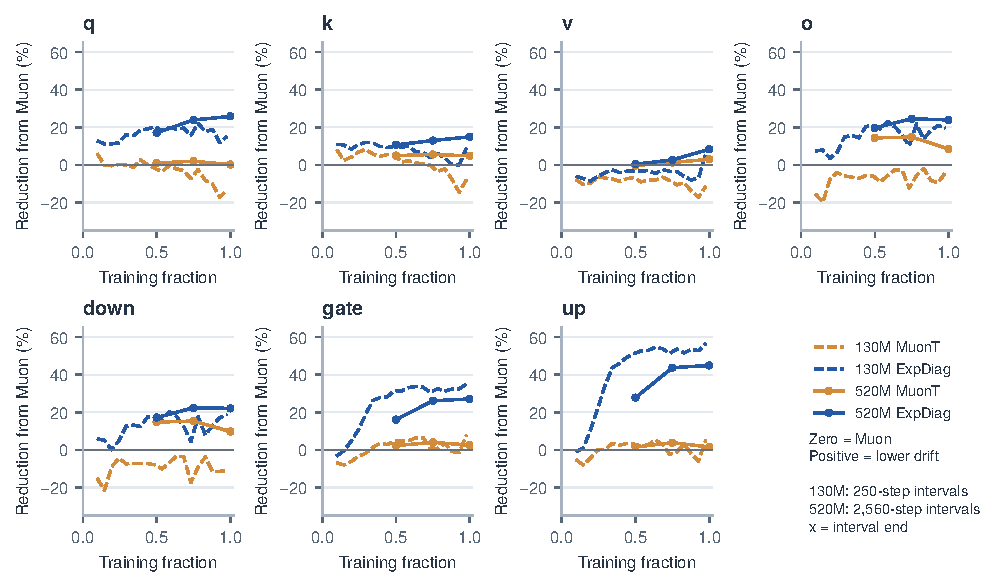
\includegraphics[width=\textwidth]{fig10_drift_by_role.pdf}
 \caption{\textbf{Fixed-data output-subspace drift reduction at each saved interval by projection role.} Curves show \mname{MuonT} and \mname{WT-MLP-Lag} relative to \mname{Muon} at the same model size and interval, averaging 32 layers and two probe sets before taking ratios (positive values denote lower drift than \mname{Muon}). Dashed curves show 130M (250-step intervals) and solid curves show 520M (2,560-step intervals, shared $\eta=0.016$) plotted against interval end as a fraction of total training steps (\Cref{tab:output_drift}).}
 \label{fig:output_drift_roles}
\end{figure}

\paragraph{Uninterrupted 130M training-EMA check.}
Separately, we compare saved dense output training EMAs ($\beta=0.938$) at every 250-step checkpoint from 250 to 5,000 between \mname{WT-MLP-Lag} and a passive \mname{MuonT} control (which records output EMAs on seed 0 at $\eta=0.02263$ while applying identity output factors; \mname{Muon} saved no output EMAs, and \mname{WT} stores only diagonals on \texttt{gate,up}, leaving the five $\dm$-wide roles \texttt{q,k,v,o,down} over 19 equal intervals plus the separate $5{,}000\text{--}5{,}120$ tail). Averaged over layers and intervals, \mname{WT} lowers top-16 EMA drift by $16.3\%,12.0\%,11.4\%,7.8\%$, and $28.0\%$ on \texttt{q,k,v,o,down}, winning $17,15,19,11$, and $17$ of $19$ intervals (\texttt{o} has higher early drift and lower late drift; because the passive control uses per-matrix updates while \mname{WT} uses batched lagged updates, this EMA check is descriptive rather than strictly causal).

\paragraph{Subspace rank, boundary-gap filtering, and finite-probe scope.}
Repeating fixed-data comparisons against \mname{Muon} at $k\in\{8,16,32,64\}$ preserves positive average reductions across all seven roles in each probe set separately at matched $\eta=0.016$—both at 520M and on all three fresh 130M seeds—whereas on the mixed-rate 130M seed-0 curve \texttt{q, k, o, down, gate, up} remain positive and \texttt{v} remains higher at every tested $k$ in each probe set. On training EMAs, \texttt{q, v, down} remain positive across all $k$, whereas \texttt{o} reverses at $k=32,64$ and \texttt{k} at $k=64$. Restricting $k=16$ comparisons to layer--interval--probe observations with relative boundary gap $(\lambda_{16}-\lambda_{17})/\lambda_{16}\ge1\%$ at both endpoints in both compared methods (retaining 47--93\% of pooled observations across roles at 130M and 52--95\% at 520M, weighted equally) preserves all sign patterns in both fixed-data and EMA audits. FP64 eigensolve residuals $\|BV-V\Lambda\|_F/\|B\|_F$ are at most $2.6\times10^{-15}$ prior to FP32 storage. Finally, finite 4,576-row probe sets do not recover exact population subspaces (for instance, at 520M the same-checkpoint top-16 distance between the two disjoint probe sets averages $0.941$ on \mname{Muon}'s \texttt{gate}, $0.924$ on \mname{MuonT}'s, and $0.750$ on \mname{WT}'s; we do not subtract this cross-set distance from temporal drift).

\FloatBarrier
\section{Learning-rate selection and complete losses}
\label{app:appendix_lr}

The short-schedule sweep uses 320 updates with a full decay schedule compressed into that 0.17B-token horizon (\Cref{tab:lr_cliff}). Whereas 320-step sweeps favor $\eta\in[0.064,0.0905]$, full 5,120-step curves achieve a strict interior minimum at $\eta^*=0.0160$ across all four core methods and degrade by $0.04\text{--}0.09$ nats when run at their 320-step argmax rates (\Cref{tab:controls,tab:lr_cliff}). Similarly, at 130M and 80 TPP, scaling from the hotter $\eta=0.02263$ rate ($\eta=0.01493$) yields $+0.00358$ nats Paloma macro difference from \mname{MuonT} versus $-0.00566$ nats at the matched horizon-scaled rate $\eta=0.01056$ (\Cref{tab:absolute_results}), underscoring how learning-rate mismatch can flip apparent second-side conclusions. Complete absolute losses and replicates at both $\eta=0.01600$ and $\eta=0.02263$—across fresh 130M seeds 1--3 and all four 520M methods, where every 520M optimizer achieves lower held-out and C4 loss at $0.01600$—appear in \Cref{tab:absolute_results,tab:seeds}.

\begin{table}[tbp]\centering\footnotesize
\setlength{\tabcolsep}{5.2pt}
\caption{\textbf{Short-schedule (320-step) versus full-budget (5,120-step) matrix learning-rate sweeps at 130M (seed 0).} Entries are final held-out losses $\Lsel$ in nats; bold marks each row's minimum within that horizon. All four core full-budget curves achieve an interior minimum at $0.0160$, whereas the compressed 320-step schedule shifts apparent optima $4\text{--}6\times$ higher.}\label{tab:lr_cliff}
\begin{tabularx}{\textwidth}{@{}>{\raggedright\arraybackslash}Xrrrrrrrr@{}}
\toprule
Method & 0.0113 & 0.0160 & 0.0226 & 0.0320 & 0.0453 & 0.0640 & 0.0905 & 0.1280 \\
\midrule
\addlinespace[2pt]\multicolumn{9}{@{}l}{\textit{Short-schedule proxy sweep: 320 steps (0.17B tokens, seed 0)}}\\
MuonT & --- & 4.5661 & 4.4221 & 4.3347 & 4.2720 & \textbf{4.2510} & 4.2533 & 4.3021 \\
Muon2-Diag & --- & 4.5787 & 4.4312 & 4.3326 & 4.2577 & 4.2339 & \textbf{4.2314} & 4.2693 \\
Abl-OuterDiag & --- & 4.5854 & 4.4417 & 4.3337 & 4.2702 & 4.2442 & \textbf{4.2367} & 4.2798 \\
Abl-OuterDiag-F & --- & 4.5887 & 4.4412 & 4.3346 & 4.2748 & \textbf{4.2411} & 4.2436 & 4.2878 \\
\addlinespace[5pt]\multicolumn{9}{@{}l}{\textit{Full-budget verification: 5,120 steps (2.68B tokens, seed 0)}}\\
Muon & 3.2496 & \textbf{3.2461} & 3.2524 & 3.2667 & --- & --- & --- & --- \\
MuonT & 3.2404 & \textbf{3.2342} & 3.2354 & 3.2398 & --- & 3.2775 & --- & --- \\
Muon2-Diag & 3.2383 & \textbf{3.2318} & 3.2333 & 3.2403 & --- & --- & 3.3200 & --- \\
Abl-OuterDiag-F & --- & --- & \textbf{3.2318} & --- & --- & 3.2752 & --- & --- \\
\rowcolor{rowtint}[0pt][0pt]\textbf{Muon2-ExpDiag} & 3.2363 & \textbf{3.2303} & 3.2311 & 3.2356 & --- & --- & --- & --- \\
\bottomrule\end{tabularx}
\end{table}

\begin{table}[tbp]\centering\scriptsize
\setlength{\tabcolsep}{8.5pt}
\caption{\textbf{Complete absolute losses and learning rates across all confirmatory regimes.} All losses are cross-entropy in nats; Late-11 Held-out averages the 11 second-half evaluation checkpoints. Hotter-LR rows ($\eta=0.02263$ at 130M and 520M 20 TPP; $\eta=0.01493$ at 130M 80 TPP) document the two-rate checks and learning-rate sensitivity discussed in \Cref{sec:phase2,sec:phase3,sec:phase4}.}\label{tab:absolute_results}
\begin{tabularx}{\textwidth}{@{}>{\raggedright\arraybackslash}Xrrrrr@{}}
\toprule
Method & Matrix $\eta$ & Final Held-out & Late-11 Held-out & Final C4 & Paloma Macro \\
\midrule
\addlinespace[2pt]\multicolumn{6}{@{}l}{\textit{130M seed-0 controls: 20 TPP, 2.68B tokens (complete learning-rate bracket)}}\\
Muon & 0.01131 & 3.2496 & 3.3692 & 3.4661 & 3.4179 \\
MuonT & 0.01131 & 3.2404 & 3.3521 & 3.4589 & 3.4154 \\
Muon2-Diag & 0.01131 & 3.2383 & 3.3500 & 3.4569 & 3.4115 \\
Muon2-ExpDiag & 0.01131 & 3.2363 & 3.3476 & 3.4548 & 3.4088 \\
Muon & 0.01600 & 3.2461 & 3.3824 & 3.4618 & --- \\
MuonT & 0.01600 & 3.2342 & 3.3591 & 3.4511 & 3.4041 \\
Muon2-Diag & 0.01600 & 3.2318 & 3.3555 & 3.4475 & 3.4048 \\
Muon2-ExpDiag & 0.01600 & 3.2303 & 3.3544 & 3.4472 & 3.3985 \\
Muon & 0.02263 & 3.2524 & 3.4064 & 3.4675 & --- \\
MuonT & 0.02263 & 3.2354 & 3.3763 & 3.4511 & 3.4021 \\
Null-Ctrl & 0.02263 & 3.2351 & 3.3755 & 3.4506 & --- \\
Muon2-Diag & 0.02263 & 3.2333 & 3.3724 & 3.4489 & --- \\
Muon2-ExpDiag & 0.02263 & 3.2311 & 3.3716 & 3.4491 & 3.4019 \\
Muon & 0.03200 & 3.2667 & 3.4426 & 3.4819 & 3.4313 \\
MuonT & 0.03200 & 3.2398 & 3.3970 & 3.4563 & --- \\
Muon2-Diag & 0.03200 & 3.2403 & 3.3981 & 3.4563 & --- \\
Muon2-ExpDiag & 0.03200 & 3.2356 & 3.3947 & 3.4533 & --- \\
\addlinespace[4pt]\multicolumn{6}{@{}l}{\textit{130M confirmation: 20 TPP, 2.68B tokens (mean of fresh seeds 1--3; matched $\eta^*$ \& hotter LR)}}\\
Muon & 0.01600 & 3.2035 & 3.3375 & 3.4640 & 3.4164 \\
MuonT & 0.01600 & 3.1916 & 3.3143 & 3.4523 & 3.4049 \\
Muon2-Diag & 0.01600 & 3.1919 & 3.3146 & 3.4514 & 3.4036 \\
\rowcolor{rowtint}[0pt][0pt]Muon2-ExpDiag & 0.01600 & 3.1881 & 3.3107 & 3.4484 & 3.4005 \\
Muon2-Diag (hotter LR) & 0.02263 & 3.1911 & 3.3282 & 3.4493 & 3.4040 \\
Muon2-ExpDiag (hotter LR) & 0.02263 & 3.1883 & 3.3265 & 3.4488 & 3.4009 \\
\addlinespace[4pt]\multicolumn{6}{@{}l}{\textit{130M longer training: 80 TPP, 10.74B tokens, seed 0 (matched \& hotter rates)}}\\
Muon & 0.01056 & 3.0778 & 3.2236 & 3.2989 & 3.2479 \\
MuonT & 0.01056 & 3.0675 & 3.2013 & 3.2886 & 3.2368 \\
Muon2-Diag & 0.01056 & 3.0656 & 3.1997 & 3.2861 & 3.2342 \\
\rowcolor{rowtint}[0pt][0pt]Muon2-ExpDiag & 0.01056 & 3.0636 & 3.1967 & 3.2848 & 3.2312 \\
Muon2-ExpDiag (hotter LR) & 0.01493 & 3.0696 & 3.2203 & 3.2900 & 3.2404 \\
\addlinespace[4pt]\multicolumn{6}{@{}l}{\textit{520M width transfer: 20 TPP, 10.74B tokens, seed 0 (matched $\eta^*$ \& hotter rates)}}\\
Muon & 0.01600 & 2.8528 & 2.9858 & 3.0769 & 3.0291 \\
MuonT & 0.01600 & 2.8438 & 2.9658 & 3.0696 & 3.0256 \\
Muon2-Diag & 0.01600 & 2.8433 & 2.9638 & 3.0674 & 3.0262 \\
\rowcolor{rowtint}[0pt][0pt]Muon2-ExpDiag & 0.01600 & 2.8392 & 2.9611 & 3.0653 & 3.0179 \\
Muon (hotter LR) & 0.02263 & 2.8639 & 3.0153 & 3.0860 & 3.0379 \\
MuonT (hotter LR) & 0.02263 & 2.8463 & 2.9839 & 3.0704 & 3.0256 \\
Muon2-Diag (hotter LR) & 0.02263 & 2.8469 & 2.9845 & 3.0708 & 3.0261 \\
Muon2-ExpDiag (hotter LR) & 0.02263 & 2.8435 & 2.9809 & 3.0682 & 3.0202 \\
\bottomrule\end{tabularx}
\end{table}

\begin{table}[tbp]\centering\footnotesize
\setlength{\tabcolsep}{7.5pt}
\caption{\textbf{Individual fresh-seed replication at 130M (20 TPP, 2.68B tokens).} Subheaders report each seed's absolute Muon losses ($\eta^*=0.01600$); rows report paired differences from same-seed Muon in millinats (negative favors the row method; Late-11 is omitted for $\eta=0.02263$ rows because intermediate decay schedules differ). Muon2-ExpDiag improves over both Muon and MuonT on every seed across all evaluation suites at both learning rates.}\label{tab:seeds}
\begin{tabularx}{\textwidth}{@{}>{\raggedright\arraybackslash}Xrrrrr@{}}
\toprule
Method & Matrix $\eta$ & $\Delta$ Held-out & Late-11 $\Delta$ & $\Delta$ C4 & $\Delta$ Paloma \\
\midrule
\addlinespace[2pt]\multicolumn{6}{@{}l}{\textit{Seed 1: Muon reference ($\Lsel=3.2003$, Late-11 $=3.3362$, $\Lc=3.4655$, $\Lpal=3.4162$ nats)}}\\
MuonT & 0.01600 & $-12.44$ & $-24.87$ & $-12.66$ & $-11.64$ \\
Muon2-Diag & 0.01600 & $-11.83$ & $-24.08$ & $-13.10$ & $-11.90$ \\
\rowcolor{rowtint}[0pt][0pt]\textbf{Muon2-ExpDiag} & 0.01600 & $\mathbf{-14.02}$ & $\mathbf{-26.50}$ & $\mathbf{-16.18}$ & $\mathbf{-15.69}$ \\
Muon2-Diag (hotter LR) & 0.02263 & $-13.46$ & --- & $-16.73$ & $-14.26$ \\
Muon2-ExpDiag (hotter LR) & 0.02263 & $-15.31$ & --- & $-17.01$ & $-15.99$ \\
\addlinespace[4pt]\multicolumn{6}{@{}l}{\textit{Seed 2: Muon reference ($\Lsel=3.1764$, Late-11 $=3.3089$, $\Lc=3.4639$, $\Lpal=3.4182$ nats)}}\\
MuonT & 0.01600 & $-12.97$ & $-23.99$ & $-11.98$ & $-15.59$ \\
Muon2-Diag & 0.01600 & $-12.58$ & $-23.61$ & $-13.55$ & $-14.99$ \\
\rowcolor{rowtint}[0pt][0pt]\textbf{Muon2-ExpDiag} & 0.01600 & $\mathbf{-17.93}$ & $\mathbf{-29.22}$ & $\mathbf{-17.11}$ & $\mathbf{-17.68}$ \\
Muon2-Diag (hotter LR) & 0.02263 & $-12.99$ & --- & $-14.58$ & $-10.86$ \\
Muon2-ExpDiag (hotter LR) & 0.02263 & $-15.21$ & --- & $-15.43$ & $-16.75$ \\
\addlinespace[4pt]\multicolumn{6}{@{}l}{\textit{Seed 3: Muon reference ($\Lsel=3.2339$, Late-11 $=3.3675$, $\Lc=3.4627$, $\Lpal=3.4148$ nats)}}\\
MuonT & 0.01600 & $-10.33$ & $-20.92$ & $-10.73$ & $-7.25$ \\
Muon2-Diag & 0.01600 & $-10.44$ & $-21.04$ & $-11.25$ & $-11.48$ \\
\rowcolor{rowtint}[0pt][0pt]\textbf{Muon2-ExpDiag} & 0.01600 & $\mathbf{-14.27}$ & $\mathbf{-24.63}$ & $\mathbf{-13.63}$ & $\mathbf{-14.35}$ \\
Muon2-Diag (hotter LR) & 0.02263 & $-10.91$ & --- & $-12.77$ & $-12.02$ \\
Muon2-ExpDiag (hotter LR) & 0.02263 & $-15.32$ & --- & $-13.42$ & $-13.78$ \\
\bottomrule\end{tabularx}
\end{table}


\FloatBarrier
\section{Placement ablations}
\label{app:ablations}

\Cref{tab:ablations_full} reports all 19 exploratory factor-placement, exponent, and scheduling arms at 130M alongside each arm's same-wave \mname{MuonT} reference. Because earlier waves (W0--W3, W10) precede the unified fast-lag confirmation runner, cross-wave comparisons are exploratory; the matched-path controls and multi-seed confirmation runs in \Cref{sec:scaling,sec:falsification} provide the primary test of \mname{WT-MLP-Lag}.

\begin{table}[tbp]\centering\footnotesize
\setlength{\tabcolsep}{3.1pt}
\caption{\textbf{Complete 19-arm placement and operator ledger at 130M (seed 0, 2.68B tokens).} Cohort identifies the implementation wave providing each arm's paired MuonT reference (W0--W4, W10, or FastLag); loss columns report cohort-adjusted differences (millinats) relative to Muon ($\text{arm}-\text{cohort MuonT}$ shifted by W0 MuonT minus Muon, which equals raw difference from Muon on W0--W4; Late averages 11 second-half checkpoints; Train averages the final 537M tokens). Step $\Delta t$ is median overhead relative to Muon in the unified 8-GPU benchmark. Because earlier waves precede the unified confirmation runner, cross-wave differences are exploratory.}\label{tab:ablations_full}
\begin{tabularx}{\textwidth}{@{}>{\raggedright\arraybackslash}Xlllrrrrr@{}}
\toprule
& & ($\dm/\dff$) & ($\dm/\dff$) & \multicolumn{4}{c}{$\Delta$ vs.\ Muon (mnats, $\downarrow$)} & \\
\cmidrule(lr){5-8}
Method & Cohort & Inputs & Outputs & Final & Late & Late C4 & Train & Step $\Delta t$ \\
\midrule
\addlinespace[2pt]\multicolumn{9}{@{}l}{\textit{Reference baselines and execution-path control}}\\
Muon & W0 & $I$ / $I$ & $I$ / $I$ & $+0.00$ & $+0.00$ & $+0.00$ & $+0.00$ & $+0.0\%$ \\
MuonT & W0 & Dense / Dense & $I$ / $I$ & $-9.48$ & $-5.50$ & $-5.34$ & $-6.16$ & $+1.5\%$ \\
Null-Ctrl & W3 & Dense / Dense & $I$ / $I$ (solved) & $-10.82$ & $-6.15$ & $-7.39$ & $-6.85$ & $+13.9\%$ \\
Null-Dense & W1 & Dense / Dense & $I$ / $I$ (solved) & $-10.65$ & $-6.79$ & $-7.64$ & $-7.52$ & $+27.5\%$ \\
Null-Diag & W10 & Dense / Dense & $I$ / $I$ (solved) & $-10.89$ & $-7.51$ & $-6.57$ & $-7.30$ & $+2.9\%$ \\
\addlinespace[4pt]\multicolumn{9}{@{}l}{\textit{Replacing or weakening input whitening}}\\
Abl-BothDiag & W1 & Diag / Diag & Diag / Diag & $-2.15$ & $+12.51$ & $+12.34$ & $+7.21$ & $+1.1\%$ \\
Abl-OutOnly & W1 & $I$ / $I$ & Dense / Dense & $-6.23$ & $+3.20$ & $+5.55$ & $+1.71$ & $+31.7\%$ \\
Abl-DownSwap & W0 & Dense / $I$ & $I$ (\texttt{down} Dense) & $-8.42$ & $-2.99$ & $-1.74$ & $-2.98$ & $+1.8\%$ \\
Abl-SymDiag (sync) & FastLag & Dense / Diag & Dense / Diag & $-12.48$ & $-8.02$ & $-7.37$ & $-7.42$ & $+10.9\%$ \\
Abl-SymDiag & FastLag & Dense / Diag & Dense / Diag & $-11.94$ & $-6.63$ & $-6.95$ & $-7.64$ & $+4.8\%$ \\
\addlinespace[4pt]\multicolumn{9}{@{}l}{\textit{Output projection role and inner/outer exponent placement}}\\
Abl-DownOnly & W0 & Dense / Dense & $\hat L_{\rm down}$ only & $-10.76$ & $-6.87$ & $-6.13$ & $-7.32$ & $+3.6\%$ \\
Abl-OuterDiag & W10 & Dense / Dense & $\hat L$ Diag / $\hat L$ Diag & $-11.27$ & $-7.96$ & $-7.94$ & $-7.54$ & $+3.0\%$ \\
Abl-NoExp & W2 & Dense / Dense & Dense / $I$ & $-12.59$ & $-8.57$ & $-7.97$ & $-8.29$ & $+13.7\%$ \\
Abl-OuterDense & W2 & Dense / Dense & $\hat L$ Dense ($L=I$) & $-13.67$ & $-9.48$ & $-10.12$ & $-10.04$ & $+28.2\%$ \\
Muon2-Diag & W2 & Dense / Dense & Diag / Diag & $-13.62$ & $-10.01$ & $-8.95$ & $-9.85$ & $+3.7\%$ \\
\addlinespace[4pt]\multicolumn{9}{@{}l}{\textit{Dense two-sided ceiling versus expansion-diagonal outputs and one-step lag}}\\
Muon2-Dense & W1 & Dense / Dense & Dense / Dense & $-15.63$ & $-11.29$ & $-11.72$ & $-11.14$ & $+23.3\%$ \\
Muon2-Dense (lag) & W3 & Dense / Dense & Dense / Dense & $-15.69$ & $-11.40$ & $-11.21$ & $-11.89$ & $+18.2\%$ \\
Muon2-ExpDiag (sync) & W2 & Dense / Dense & Dense / Diag & $\mathbf{-16.37}$ & $\mathbf{-12.09}$ & $-11.42$ & $-11.23$ & $+12.9\%$ \\
\rowcolor{rowtint}[0pt][0pt]\textbf{Muon2-ExpDiag} & W4 & Dense / Dense & Dense / Diag & $\mathbf{-16.04}$ & $\mathbf{-11.19}$ & $\mathbf{-10.33}$ & $\mathbf{-11.11}$ & $+6.8\%$ \\
\bottomrule\end{tabularx}
\end{table}


\FloatBarrier
\section{Systems measurements and domain evaluation}
\label{app:appendix_systems}

The unified 130M timing benchmark (\Cref{tab:bench19}) initializes all 19 arms from identical step-2,500 weights with fresh optimizer/moment state on $8\times\text{A100}$, warms up for 36 steps, and records rank-0 real-data training step durations over steps 37--96 (including data loading and distributed gradient synchronization, excluding compilation, evaluation, and checkpoint I/O). One 60-step window per arm does not resolve sub-percent differences or per-rank maxima. The 520M records (\Cref{tab:bench520m}) report complete windows without outlier removal across both matched-checkpoint initialization (steps 37--96) and each method's own warmed step-5,120 optimizer state (steps 17--76) on $8\times$ and $32\times\text{A100}$ GPUs. Complete 16-domain Paloma scores appear in \Cref{tab:paloma_full}.

\begin{table}[tbp]\centering\footnotesize
\setlength{\tabcolsep}{9.5pt}
\caption{\textbf{Complete 19-arm 130M timing and memory benchmark on 8$\times$A100.} Sorted by median step duration over steps 37--96 (after 36 warmup steps) from identical step-2,500 weights and fresh optimizer/moment state. Both median and mean overheads ($\Delta$) are relative to Muon.}\label{tab:bench19}
\begin{tabularx}{\textwidth}{@{}>{\raggedright\arraybackslash}Xrrrrr@{}}
\toprule
Method & Median (s) & Median $\Delta$ & Mean (s) & Mean $\Delta$ & Peak GiB \\
\midrule
Muon & 1.0810 & $+0.0\%$ & 1.0792 & $+0.0\%$ & 18.97 \\
Abl-BothDiag & 1.0926 & $+1.1\%$ & 1.0911 & $+1.1\%$ & 19.55 \\
MuonT & 1.0967 & $+1.5\%$ & 1.0971 & $+1.7\%$ & 20.54 \\
Abl-DownSwap & 1.1005 & $+1.8\%$ & 1.0976 & $+1.7\%$ & 19.41 \\
Null-Diag & 1.1121 & $+2.9\%$ & 1.1121 & $+3.0\%$ & 20.55 \\
Abl-OuterDiag & 1.1131 & $+3.0\%$ & 1.1134 & $+3.2\%$ & 20.55 \\
Abl-DownOnly & 1.1202 & $+3.6\%$ & 1.1283 & $+4.5\%$ & 20.76 \\
Muon2-Diag & 1.1211 & $+3.7\%$ & 1.1196 & $+3.7\%$ & 20.55 \\
Abl-SymDiag & 1.1331 & $+4.8\%$ & 1.1751 & $+8.9\%$ & 20.82 \\
\rowcolor{rowtint}[0pt][0pt]\textbf{Muon2-ExpDiag} & 1.1548 & $+6.8\%$ & 1.1944 & $+10.7\%$ & 21.60 \\
Abl-SymDiag (sync) & 1.1986 & $+10.9\%$ & 1.2356 & $+14.5\%$ & 20.74 \\
Muon2-ExpDiag (sync) & 1.2208 & $+12.9\%$ & 1.2501 & $+15.8\%$ & 21.52 \\
Abl-NoExp & 1.2288 & $+13.7\%$ & 1.2517 & $+16.0\%$ & 21.52 \\
Null-Ctrl & 1.2313 & $+13.9\%$ & 1.2493 & $+15.8\%$ & 21.52 \\
Muon2-Dense (lag) & 1.2782 & $+18.2\%$ & 1.4585 & $+35.1\%$ & 24.78 \\
Muon2-Dense & 1.3333 & $+23.3\%$ & 1.4595 & $+35.2\%$ & 24.21 \\
Null-Dense & 1.3785 & $+27.5\%$ & 1.4638 & $+35.6\%$ & 24.21 \\
Abl-OuterDense & 1.3861 & $+28.2\%$ & 1.5004 & $+39.0\%$ & 24.21 \\
Abl-OutOnly & 1.4232 & $+31.7\%$ & 1.4579 & $+35.1\%$ & 22.21 \\
\bottomrule\end{tabularx}
\end{table}

\begin{table}[tbp]\centering\footnotesize
\setlength{\tabcolsep}{9.5pt}
\caption{\textbf{Complete 520M timing and memory records across 8 and 32 A100 GPUs (1.0M batch, chunked buffers).} All rows report the complete recorded measurement window without outlier removal; own optimizer states restore each arm's converged step-5,120 moments and eigenbases. Overheads ($\Delta$) are relative to within-group Muon.}\label{tab:bench520m}
\begin{tabularx}{\textwidth}{@{}>{\raggedright\arraybackslash}Xrrrrr@{}}
\toprule
Method & Median (s) & Median $\Delta$ & Mean (s) & Mean $\Delta$ & Peak GiB \\
\midrule
\addlinespace[2pt]\multicolumn{6}{@{}l}{\textit{8 GPUs, matched checkpoint, steps 37--96}}\\
Muon & 4.6419 & $+0.0\%$ & 4.6456 & $+0.0\%$ & 26.46 \\
MuonT & 4.8943 & $+5.4\%$ & 4.9010 & $+5.5\%$ & 29.05 \\
Muon2-Diag & 4.9863 & $+7.4\%$ & 4.9902 & $+7.4\%$ & 29.06 \\
\rowcolor{rowtint}[0pt][0pt]\textbf{Muon2-ExpDiag} & 5.3219 & $+14.6\%$ & 5.3181 & $+14.5\%$ & 30.73 \\
\addlinespace[4pt]\multicolumn{6}{@{}l}{\textit{32 GPUs, matched checkpoint, steps 37--96}}\\
Muon & 1.3222 & $+0.0\%$ & 1.3241 & $+0.0\%$ & 26.46 \\
MuonT & 1.3851 & $+4.8\%$ & 1.3911 & $+5.1\%$ & 26.93 \\
Muon2-Diag & 1.4063 & $+6.4\%$ & 1.4119 & $+6.6\%$ & 26.94 \\
\rowcolor{rowtint}[0pt][0pt]\textbf{Muon2-ExpDiag} & 1.4305 & $+8.2\%$ & 1.5493 & $+17.0\%$ & 27.88 \\
\addlinespace[4pt]\multicolumn{6}{@{}l}{\textit{32 GPUs, own optimizer states, steps 17--76}}\\
Muon & 1.3124 & $+0.0\%$ & 1.3163 & $+0.0\%$ & 26.46 \\
MuonT & 1.3809 & $+5.2\%$ & 1.3853 & $+5.2\%$ & 26.93 \\
Muon2-Diag & 1.4203 & $+8.2\%$ & 1.4453 & $+9.8\%$ & 26.94 \\
\rowcolor{rowtint}[0pt][0pt]\textbf{Muon2-ExpDiag} & 1.4578 & $+11.1\%$ & 1.5388 & $+16.9\%$ & 27.88 \\
\addlinespace[4pt]\multicolumn{6}{@{}l}{\textit{8 GPUs, own optimizer states, steps 17--76}}\\
Muon & 4.6383 & $+0.0\%$ & 4.6396 & $+0.0\%$ & 26.46 \\
MuonT & 4.8779 & $+5.2\%$ & 4.8994 & $+5.6\%$ & 29.05 \\
Muon2-Diag & 5.0287 & $+8.4\%$ & 5.0533 & $+8.9\%$ & 29.07 \\
\rowcolor{rowtint}[0pt][0pt]\textbf{Muon2-ExpDiag} & 5.6081 & $+20.9\%$ & 5.6098 & $+20.9\%$ & 30.74 \\
\bottomrule\end{tabularx}
\end{table}

\begin{table}[tbp]\centering\small
\setlength{\tabcolsep}{7.0pt}
\caption{\textbf{Per-domain Paloma loss differences from MuonT across all 16 domains.} Entries are millinats ($\text{Method}-\text{MuonT}$; negative favors the method, bold marks the stronger output approximation within each regime). The 130M 20-TPP columns average paired differences across fresh seeds 1--3; 130M 80-TPP and 520M 20-TPP use single-seed matched-rate runs.}\label{tab:paloma_full}
\begin{tabularx}{\textwidth}{@{}>{\raggedright\arraybackslash}Xrrrrrr@{}}
\toprule
& \multicolumn{2}{c}{130M, 20 TPP (3 seeds)} & \multicolumn{2}{c}{130M, 80 TPP} & \multicolumn{2}{c}{520M, 20 TPP} \\
\cmidrule(lr){2-3}\cmidrule(lr){4-5}\cmidrule(lr){6-7}
Paloma domain & OD-All & WT-Lag & OD-All & WT-Lag & OD-All & WT-Lag \\
\midrule
C4-EN & $-0.85$ & $\mathbf{-3.86}$ & $-2.55$ & $\mathbf{-3.80}$ & $-2.14$ & $\mathbf{-4.27}$ \\
C4 domains & $-0.98$ & $\mathbf{-3.78}$ & $-1.85$ & $\mathbf{-4.07}$ & $-0.98$ & $\mathbf{-2.92}$ \\
mC4 & $+0.29$ & $\mathbf{-3.73}$ & $-1.08$ & $\mathbf{-2.66}$ & $-2.76$ & $\mathbf{-6.36}$ \\
Dolma & $-1.12$ & $\mathbf{-4.13}$ & $-2.23$ & $\mathbf{-4.35}$ & $-1.95$ & $\mathbf{-3.58}$ \\
RefinedWeb & $-1.10$ & $\mathbf{-3.96}$ & $-3.43$ & $\mathbf{-5.00}$ & $-1.99$ & $\mathbf{-3.63}$ \\
RedPajama & $-0.73$ & $\mathbf{-2.81}$ & $-3.63$ & $\mathbf{-4.11}$ & $-1.75$ & $\mathbf{-8.12}$ \\
Wikipedia & $-0.75$ & $\mathbf{-3.88}$ & $-2.51$ & $\mathbf{-4.80}$ & $-0.00$ & $\mathbf{-2.36}$ \\
S2ORC & $-0.51$ & $\mathbf{-4.35}$ & $-3.11$ & $\mathbf{-4.78}$ & $-0.67$ & $\mathbf{-3.93}$ \\
Programming & $+0.51$ & $\mathbf{-4.29}$ & $-0.77$ & $\mathbf{-0.91}$ & $-2.11$ & $\mathbf{-5.39}$ \\
WikiText-103 & $\mathbf{+2.05}$ & $+2.84$ & $-6.14$ & $\mathbf{-11.00}$ & $+4.43$ & $\mathbf{-2.16}$ \\
Penn Treebank & $\mathbf{-9.42}$ & $-1.52$ & $-15.72$ & $\mathbf{-19.42}$ & $-0.15$ & $\mathbf{-7.17}$ \\
Subreddits & $+0.62$ & $\mathbf{-1.85}$ & $\mathbf{-3.34}$ & $-3.03$ & $-2.32$ & $\mathbf{-3.84}$ \\
TwitterAAE & $-6.94$ & $\mathbf{-19.72}$ & $+18.06$ & $\mathbf{-2.21}$ & $+8.74$ & $\mathbf{-59.67}$ \\
Manosphere & $-1.50$ & $\mathbf{-7.05}$ & $-0.57$ & $\mathbf{-1.46}$ & $-2.22$ & $\mathbf{-5.87}$ \\
4chan & $+2.33$ & $\mathbf{-3.40}$ & $-7.74$ & $\mathbf{-9.18}$ & $+3.44$ & $\mathbf{-2.78}$ \\
Gab & $-2.62$ & $\mathbf{-5.16}$ & $-4.86$ & $\mathbf{-9.87}$ & $+13.00$ & $\mathbf{-0.04}$ \\
\midrule
\rowcolor{rowtint}[0pt][0pt]\textbf{16-domain macro mean} & $-1.30$ & $\mathbf{-4.41}$ & $-2.59$ & $\mathbf{-5.66}$ & $+0.66$ & $\mathbf{-7.63}$ \\
\textbf{Domains won vs.\ MuonT} & 11/16 & \textbf{15/16} & 15/16 & \textbf{16/16} & 12/16 & \textbf{16/16} \\
\bottomrule\end{tabularx}
\end{table}



\end{document}
